% \documentclass{article}
% %\documentclass[hyperref={colorlinks=true}]{beamer}
% %\documentclass[handout,hyperref={colorlinks=true}]{beamer}
% 
% 
% %%%%%%%%%%%%%%%%%%%%%%%%%%%%%%Paquetes%%%%%%%%%%%%%%%%%%%%%%%%%%%%%%%%%%%%%%%%%%%%%%%5
% %%%%%%%%%%%%%%%%%%%%%%%%%%%%%%%%%%%%%%%%%%%%%%%%%%%%%%%%%%%%%%%%%%%%%%%%%%%%%%%%%%%%%
% \usepackage{empheq}
% \usepackage[spanish]{babel}
% \usepackage[utf8x]{inputenc}
% \usepackage{times}
% %\usepackage[T1]{fontenc}
% %\usepackage[latin1]{inputenc}
% \usepackage{amssymb,amsmath,amsthm}
% \usepackage{enumerate}
% \usepackage{verbatim}
% \usepackage{ esint }
% %\usepackage{pst-all}
% %\usepackage{pstricks-add}
% \usepackage{array}
% \usepackage{animate}
% %\usepackage{media9}
% \usepackage{xparse}
% \usepackage{listings}
% \usepackage{ wasysym }
% %\usepackage{sagetex}
% \usepackage{yfonts,mathrsfs,eufrak}
% \usepackage{hyperref}
% \usepackage{color}
% \usepackage{url}
% \usepackage{theorem}
% \usepackage{boiboites}
% \usepackage{wrapfig}
% \usepackage{ esint }
% \usepackage{varioref}
% \definecolor{mygreen}{rgb}{0,0.6,0}
% \definecolor{mygray}{rgb}{0.5,0.5,0.5}
% \definecolor{mymauve}{rgb}{0.58,0,0.82}
% 
% \lstset{ %
%   backgroundcolor=\color{white},   % choose the background color; you must add \usepackage{color} or \usepackage{xcolor}
%   basicstyle=\footnotesize,        % the size of the fonts that are used for the code
%   breakatwhitespace=false,         % sets if automatic breaks should only happen at whitespace
%   breaklines=true,                 % sets automatic line breaking
%   captionpos=b,                    % sets the caption-position to bottom
%   commentstyle=\color{mygreen},    % comment style
%   deletekeywords={...},            % if you want to delete keywords from the given language
%   escapeinside={\%*}{*)},          % if you want to add LaTeX within your code
%   extendedchars=true,              % lets you use non-ASCII characters; for 8-bits encodings only, does not work with UTF-8
%   frame=single,	                   % adds a frame around the code
%   keepspaces=true,                 % keeps spaces in text, useful for keeping indentation of code (possibly needs columns=flexible)
%   keywordstyle=\color{blue},       % keyword style
%   language=Python,                 % the language of the code
%   otherkeywords={*,...},           % if you want to add more keywords to the set
%   numbers=none,                    % where to put the line-numbers; possible values are (none, left, right)
%   numbersep=5pt,                   % how far the line-numbers are from the code
%   numberstyle=\tiny\color{mygray}, % the style that is used for the line-numbers
%   rulecolor=\color{black},         % if not set, the frame-color may be changed on line-breaks within not-black text (e.g. comments (green here))
%   showspaces=false,                % show spaces everywhere adding particular underscores; it overrides 'showstringspaces'
%   showstringspaces=false,          % underline spaces within strings only
%   showtabs=false,                  % show tabs within strings adding particular underscores
%   stepnumber=2,                    % the step between two line-numbers. If it's 1, each line will be numbered
%   stringstyle=\color{mymauve},     % string literal style
%   tabsize=2,	                   % sets default tabsize to 2 spaces
%   title=\lstname,                   % show the filename of files included with \lstinputlisting; also try caption instead of title
%   belowskip=-0.5cm
% }
% 
% 
% %%%%%%%%%%%%%%%%%%%%%%%%%%Nuevos comandos entornos%%%%%%%%%%%%%%%%%%%%%%%%%%%%%%%%
% %%%%%%%%%%%%%%%%%%%%%%%%%%%%%%%%%%%%%%%%%%%%%%%%%%%%%%%%%%%%%%%%%%%%%%%%
% \newenvironment{demo}{\noindent\emph{Dem.}}{$\square$ \newline\vspace{5pt}}
% 
% \newcommand{\com}{\mathbb{C}}
% \newcommand{\dis}{\mathbb{D}}
% \newcommand{\rr}{\mathbb{R}}
% \newcommand{\oo}{\mathcal{O}}
% %\renewcommand{\emph}[1]{\textcolor[rgb]{1,0,0}{#1}}
% \newcommand{\der}[2]{\frac{\partial #1}{\partial #2}}
% \renewcommand{\v}[1]{\overrightarrow{#1}}
% \renewcommand{\epsilon}{\varepsilon}
% %\newcommand{\defverbatim}{\def{#1}}
% \renewcommand{\b}[1]{\boldsymbol{#1}}
% \renewenvironment{frame}[1]{}{}
% %\newcommand{\end{proof}}{$\square$}
% \DeclareMathOperator{\atan2}{atan2}
% \DeclareMathOperator{\sen}{sen}
% 
% 
% %%%%%%%%%%%%%%%%%%%%%%%%Colores
% \definecolor{myblue}{rgb}{.8, .8, 1}
% \definecolor{dblackcolor}{rgb}{0.0,0.0,0.0}
% \definecolor{dbluecolor}{rgb}{0.01,0.02,0.7}
% \definecolor{dgreencolor}{rgb}{0.2,0.4,0.0}
% \definecolor{dgraycolor}{rgb}{0.30,0.3,0.30}
% \newcommand{\dblue}{\color{dbluecolor}\bf}
% \newcommand{\dred}{\color{dredcolor}\bf}
% \newcommand{\dblack}{\color{dblackcolor}\bf}
% 
% 
% %%%%%%%%%%Definimos una caja con color
% \newlength\mytemplen
% \newsavebox\mytempbox
% \makeatletter
% \newcommand\mybluebox{%
% \@ifnextchar[%]
% {\@mybluebox}%
% {\@mybluebox[0pt]}}
% \def\@mybluebox[#1]{%
% \@ifnextchar[%]
% {\@@mybluebox[#1]}%
% {\@@mybluebox[#1][0pt]}}
% \def\@@mybluebox[#1][#2]#3{
% \sbox\mytempbox{#3}%
% \mytemplen\ht\mytempbox
% \advance\mytemplen #1\relax
% \ht\mytempbox\mytemplen
% \mytemplen\dp\mytempbox
% \advance\mytemplen #2\relax
% \dp\mytempbox\mytemplen
% \colorbox{myblue}{\hspace{1em}\usebox{\mytempbox}\hspace{1em}}}
% \makeatother
% \DeclareDocumentCommand\boxedeq{ m g }{%
% {\begin{empheq}[box={\mybluebox[2pt][2pt]}]{equation}% #1%
% \IfNoValueF {#2} {\label{#2}}%
% #1
% \end{empheq}
% }%
% }
% 
% 
% %%%%%%%%%%%%%%%%%%
% \newboxedtheorem[boxcolor=orange, background=blue!5, titlebackground=blue!20,
% titleboxcolor = black,thcounter=section]{problema}{Problema}{thcounter1}
% 
% \newboxedtheorem[boxcolor=orange, background=blue!5, titlebackground=blue!20,
% titleboxcolor = black,thcounter=section]{teorema}{Teorema}{thcounter2}
% 
% \newboxedtheorem[boxcolor=orange, background=blue!5, titlebackground=blue!20,
% titleboxcolor = black,thcounter=section]{definicion}{Definici\'on}{thcounter3}
% 
% \newboxedtheorem[boxcolor=orange, background=blue!5, titlebackground=blue!20,
% titleboxcolor = black,thcounter=section]{lema}{Lema}{thcounter4}
% 
% \newboxedtheorem[boxcolor=orange, background=blue!5, titlebackground=blue!20,
% titleboxcolor = black,thcounter=section]{corolario}{Corolario}{thcounter5}
% 
% \newboxedtheorem[boxcolor=orange, background=blue!5, titlebackground=blue!20,
% titleboxcolor = black,thcounter=section]{proposicion}{Proposici\'on}{thcounter6}
% 
% \newboxedtheorem[boxcolor=orange, background=blue!5, titlebackground=blue!20,
% titleboxcolor = black,thcounter=section]{codigo}{Función SymPy}{}
% 
% \newboxedtheorem[boxcolor=orange, background=blue!5, titlebackground=blue!20,
% titleboxcolor = black,thcounter=section]{ejercicio}{Ejercicio}{}
% 
% 
% \newcounter{ejemplo_cont}
% \setcounter{ejemplo_cont}{1}
% 
% \newenvironment{ejemplo}{\noindent\textbf{Ejemplo  \arabic{ejemplo_cont}.} }{\addtocounter{ejemplo_cont}{1}}
% %%%%%%%%%%%%%%%%%%%%%%%%%%%%%%%%%%%%%%%%%%%%%%%%%%%%%%%%%%%%%%%%%%%%%%%%%%%%%%%%%%%%%%%%%%%%%%%%%%%%%%%%%%%
% %%%%%%%%%%Para escibir en clase articulo o similar
% 
% 
% 



\chapter[Series de Potencias y de Frobenius]{Métodos de desarrollo en serie de potencias y en serie de Frobenius}
%\date{}

%\begin{document}

%\tableofcontents


 \section{Series de potencias}

En esta sección recordamos algunos conceptos y teoremas sobre series de potencias. Dado que este tema es motivo de un estudio más profundo en otras materias de la licenciatura en matemática omitimos algunas demostraciones.
\subsection{Definición} %Primer Frame para información personal.
\begin{definicion} Una serie de potencias es una serie de la forma:
\[
	\sum\limits_{n=0}^{\infty}a_n(z-z_0)^n
\]
donde $a_n$, $n=0,1,\ldots$, $z_0$ y $z$ son elementos de $\com$.
\end{definicion}


Estamos interesados en determinar los valores de $z$ para los cuales   una serie converge.

\begin{ejemplo} La serie geométrica
\[
	\sum\limits_{n=0}^{\infty}z^n,
\]
es una serie de potencias. Aquí  $a_n=1$, $n=0,1,\ldots$ y $z_0=0$. Esta serie converge para $|z|<1$ a
\[ \frac{1}{1-z}\]
y no converge para cualquier otro valor de $z\in\com$.
\end{ejemplo}

\begin{ejemplo} Supongamos $f:I\to\rr$, donde $I$ es un intervalo abierto $I=(a,b)$ y que $f$ tiene derivadas de todo orden en  $z_0\in I$. Entonces es posible construir la serie de Taylor de $f$ en $z_0$ que es una serie de potencias. Recordemos que esta serie es
\[S(f,z_0,z)=\sum\limits_{n=0}^{\infty}\frac{f^{(n)}(z_0)}{n!}(z-z_0)^n.\]
\end{ejemplo}




\subsection{Límites superior e inferior}


\begin{definicion} Dada una sucesión de números reales $x_n$,
 consideramos una nueva sucesión:

\[
	A_n=\sup\{x_n, x_{n+1},\ldots \}
\]

La nueva sucesión de reales $A_n$ es  no creciente ($A_n\geq A_{n+1}$), luego tiene un límite (puede ser $\pm\infty$). A este límite lo llamamos \emph{el límite superior de $x_n$}. Lo denotamos por $\limsup_{n\to\infty} x_n$. Es decir:


\[
\limsup_{n\to\infty} x_n=\lim_{n\to\infty} A_n=\lim\limits_{n\to \infty} \sup\{x_n, x_{n+1},\ldots \}.
\]


Tomando ínfimo en lugar de supremo conseguimos \emph{el límite inferior} ($\liminf$).
\end{definicion}
\begin{ejemplo}  Si $x_n=(-1)^n$, entonces
\[
	\{x_n,x_{n+1},\ldots\}=\{\pm1,\mp1,\pm1,\ldots\}.
\]
El supremo de este conjunto  es para todo $n$ igual a 1 y el ínfimo igual a -1. Luego $\liminf x_n=-1$ y $\limsup x_n=1$.
\end{ejemplo}



\begin{ejemplo}  Si $x_n=1/n$, si $n$ es par y $x_n=1$ si $n$ es impar, entonces el conjunto

\[
	\{x_n,x_{n+1},\ldots\}
\]
tiene por supremo 1 y el ínfimo igual a $0$ . Luego $\liminf x_n=0$ y $\limsup x_n=1$.
\end{ejemplo}

\begin{teorema}\textbf{Propiedades} Sea $x_n$  e $y_n$ dos sucesiones de números reales, entonces:

\begin{enumerate}
	\item El $\limsup x_n$ y el $\liminf x_n$  existen si se permite que $\pm\infty$ sean sus posibles valores.
	\item $\liminf x_n \leq \limsup x_n$.
	\item $\liminf x_n=\limsup x_n$ si y solo si el $\lim x_n$ existe. En este caso todos los límites coinciden.
	\item $\liminf (x_n+y_n)\geq \liminf x_n + \liminf y_n$.
	\item $\limsup (x_n+y_n)\leq \limsup x_n + \limsup y_n$

\end{enumerate}
\end{teorema}



\subsection{Radio de convergencia}


\begin{definicion} Dada la serie de potencias
\[
	\sum\limits_{n=0}^{\infty}a_n(z-z_0)^n,
\]
definimos el \emph{radio de convergencia} $R$ de la siguiente forma:



\[
\frac{1}{R}=\limsup\limits_{n\to \infty} |a_n|^{1/n}.
\]

\end{definicion}

\begin{ejemplo} La serie
\[
	\sum\limits_{n=0}^{\infty}z^n,
\]
tiene radio de convergencia:

\[\frac{1}{R}=\limsup\limits_{n\to \infty}1^{1/n}=\lim\limits_{n\to\infty}1^{1/n}=1\]
Luego $R=1$.
\end{ejemplo}

\begin{ejemplo} La serie
\[
	\sum\limits_{n=0}^{\infty}\bigg(\frac{1}{M}\bigg)^nz^n,
\]
tiene radio de convergencia:

\[\frac{1}{R}=\limsup\limits_{n\to \infty}\bigg(\bigg(\frac{1}{M}\bigg)^n\bigg)^{1/n}=\lim\limits_{n\to\infty}\bigg(\bigg(\frac{1}{M}\bigg)^n\bigg)^{1/n}=\frac1M\]
Luego $R=M$.

\end{ejemplo}

\begin{ejemplo} Fijemos $M>0$ y $n$ un natural tal que $[n/2] >M$ (aquí $[x]$ es la parte entera de $x$). Entonces,
como $n-[n/2]\geq [n/2]>M$

\[
\begin{split}
n!=n(n-1)\cdots 1 &> n(n-1)\cdots (n-[n/2]) \\
&>\underbrace{M\cdots M }_{[n/2]-\hbox{veces}}\\
&\geq M^{[n/2]}\\
&> M^{n/3}\\
\end{split}
\]
Luego
\[\frac{1}{R}:=\limsup_{n\to\infty} (1/n!)^{1/n}\leq \lim_{n\to\infty} \bigg(\frac{1}{M^{n/3}}\bigg)^{1/n}=\frac{1}{\sqrt[3]{M}}\]
Como $M$ es arbitrario, haciendo $M\to\infty$ vemos que el radio de convergencia de la serie  $\sum\limits_{n=0}^{\infty}\frac{1}{n!}z^n$
es $R=\infty$.
\end{ejemplo}

\begin{teorema}  Supongamos que la serie:
\[
	\sum\limits_{n=0}^{\infty}a_n(z-z_0)^n,
\]
tiene radio de convergencia $R>0$. Entonces:
\begin{enumerate}
	\item Si $|z-z_0|<R$, la serie converge absolutamente en $z$.
	\item Si $|z-z_0|>R$, la serie diverge.
	\item Si $|z-z_0|=R$, no se afirma nada.

\end{enumerate}
\end{teorema}

 \begin{demo} Se puede suponer sin perdida de generalidad $z_0=0$. Supongamos $0<R<\infty$.  Sea $L=1/R$ y tomemos $\epsilon>0$ pequeño. Como
\[\lim_{n\to\infty}\sup\{|a_n|^{1/n},|a_{n+1}|^{1/n+1},\ldots\}=L\]
para $n_0$ suficientemente grande
\[\sup\{|a_n|^{1/n},|a_{n+1}|^{1/n+1},\ldots\}<L+\epsilon.\]
para $n\geq n_0$.   Así
\[|a_n|^{1/n}<L+\epsilon\quad\hbox{para } n\geq n_0.\]
Elijamos $0<r<1/(L+\epsilon)<1/L=R$. Si $|z|<r$ entonces
\[|a_n||z|^n<(L+\epsilon)^nr^n\quad\hbox{para } n\geq n_0.\]
Pero $r(L+\epsilon)<1$. La desigualdad de arriba y el teorema de comparación para series (notar que el miembro de la derecha forma una serie geométrica) implican que la serie converge absolutamente para este $z$.  Esto implica la convergencia para cualquier $|z|<R$, ya que si $|z|<R=1/L$ existe $\epsilon>0$ lo suficientemente chico para que $|z|<1/(L+\epsilon)$. Por el resultado ya demostrado la serie converge absolutamente para este $z$.\end{demo}
\begin{ejercicio} Demostrar los casos $R=0$, $R=\infty$ y el segundo inciso.
 \end{ejercicio}
\begin{teorema}  La función
\[
f(z)=	\sum\limits_{n=0}^{\infty}a_n(z-z_0)^n,
\]
es diferenciable dentro en $\{z:|z-z_0|<R\}$. Además
\[
f'(z)=g(z):=	\sum\limits_{n=1}^{\infty}na_n(z-z_0)^{n-1},
\]
teniendo esta serie el mismo radio de convergencia que el de $f$.
\end{teorema}

\begin{demo} Nuevamente supondremos $z_0=0$. La afirmación sobre el radio de convergencia es consecuencia de que $\lim_{n\to\infty}n^{1/n}=1$. Como el radio $R'$ de convergencia de $g$ es:

\[
\begin{split}
\frac{1}{R'}&=\limsup_{n\to\infty}|a_{n+1}(n+1)|^{1/(n+1)}\\
&\underbrace{=}_{\hbox{\emph{ Ejercicio}}}\limsup_{n\to\infty}|a_{n+1}|^{1/(n+1)}\lim_{n\to\infty}|(n+1)|^{1/(n+1)}\\
&=\limsup_{n\to\infty}|a_{n+1}|^{1/(n+1)}=\frac{1}{R}
\end{split}\]

Ahora veamos que  $f'=g$.   Sea $0<r<R$, $|z_0|<r$ y $N\in\mathbb{N}$. Pongamos:
\[f(z)=S_N(z)+E_N(z),\]
\[S_N(z)=\sum_{n=0}^{N}a_nz^n\quad\hbox{y}\quad E_N(z)=\sum_{n=N+1}^{\infty}a_nz^n\]
Tomemos $|h|<r-|z_0|$, así $|z_0+h|<r$.  Tenemos
\[\begin{split}
\frac{f(z_0+h)-f(z_0)}{h}-g(z_0)&= \frac{S_N(z_0+h)-S_N(z_0)}{h}-S_N'(z_0)\\
				&+S_N'(z_0)-g(z_0)\\
				&+\frac{E_N(z_0+h)-E_N(z_0)}{h}
\end{split}\]

Ahora si $\epsilon>0$

\[\begin{split}
				&\bigg|\frac{E_N(z_0+h)-E_N(z_0)}{h}\bigg|\leq\sum_{n=N+1}^{\infty}|a_n|\bigg|\frac{(z_0+h)^n-z_0^n}{h}\bigg|\\
				&=\sum_{n=N+1}^{\infty}|a_n|(|z_0|^{n-1}+|z_0|^{n-2}h+\cdots+h^{n-1})\\
				&\leq2\sum_{n=N+1}^{\infty}|a_n|nr^{n-1}<\epsilon\\
\end{split}\]
Para $N$ suficientemente grande. Además como $S_N'(z)\to g(z)$ cuando $N\to\infty$ podemos elegir, a su vez, $N$ suficientemente grande para que

\[
	|S_N'(z_0)-g(z_0)|<\epsilon
\]

 Fijemos un $N$ que satisfaga las condiciones anteriores. Ahora podemos encontrar $\delta>0$ para que $|h|<\delta$ cumpla que
\[
\bigg|\frac{S_N(z_0+h)-S_N(z_0)}{h}-S_N'(z_0)\bigg|<\epsilon.
\]

Esto muestra que $f'(z_0)=g(z_0)$ y por consiguiente $f$ es derivavble.
\end{demo}





\begin{corolario}  Una serie de potencias es infinitamente diferenciable. Las sucesivas derivadas se obtienen derivando término a término la serie. El radio de convergencia se conserva.
\end{corolario}

\begin{ejemplo}  Hemos visto que la serie:
\[
	f(z)=\sum_{n=0}^{\infty}\frac{1}{n!}z^n
\]
tiene radio de convergencia infinito y por ende converge en $\com$. Ahora vemos que
\[f'(z)=\sum_{n=1}^{\infty}\frac{1}{(n-1)!}z^{n-1} =\sum_{n=0}^{\infty}\frac{1}{n!}z^n
\]
Lo que nos dice que $f$ resuelve la simple ecuación diferencial $f'(z)=f(z)$. La misma ecuación es resuelta por $g(z)=e^z$. Además $f(0)=g(0)=1$. Por el Teorema de existencia y unicidad $f(z)=g(z)$ para todo $z$. Hemos probado la importante fórmula.
\boxedeq{e^z=\sum_{n=0}^{\infty}\frac{1}{n!}z^n}{eq:exp}
\end{ejemplo}
\subsection{Funciones analíticas}
\begin{definicion} Una función $f:\Omega\subset\com\to\com$ se dirá analítica si para cada $z_0\in\Omega$, existe  $R>0$ y $a_n\in\com$, tal que:

\[ f(z)=\sum_{n=0}^{\infty}a_n(z-z_0)^n,\quad\hbox{para } |z-z_0|<R \]
\end{definicion}


\begin{ejercicio} Si $f$ es analítica tenemos la siguiente fórmula
\[
	a_n=\frac{f^{(n)}(z_0)}{n!}
\]
para los coeficientes $a_n$.
\end{ejercicio}

 \begin{teorema}\label{teor_oper_series}\textbf{Operaciones entre series de potencias} Supongamos que $f(z)=\sum_{n=0}^{\infty}a_n(z-z_0)^n$ y  $g(z)=\sum_{n=0}^{\infty}b_n(z-z_0)^n$ son series de potencias con radio de convergencia mayor o igual a $R>0$. Entonces $f+g$ y $fg$ son funciones analíticas que tienen por desarrollo en serie
\[
    \begin{split}
      (f+g)(z)&=\sum_{n=0}^{\infty}(a_n+b_n)(z-z_0)^n\\
      (fg)(z)&=\sum_{n=0}^{\infty}\left(\sum_{k=0}^na_kb_{n-k}\right)(z-z_0)^n,\\
    \end{split}
\]
y los radios de convergencia de las series anteriores es, al menos, $R$. Si $g(z)\neq 0$ para $|z-z_0|<R$ entonces $f(z)/g(z)$ es analítica y se desarrolla por  una  serie de radio de convergencia al menos $R$. Es posible expresar los coeficientes del cociente en términos de los coeficientes del dividendo y divisor, pero no nos detendremos en ello.
\end{teorema}


\section{Solución de EDO mediante series de potencias. Método coeficientes indeterminados}



\subsection{Método coeficientes indeterminados}

Dada una EDO

\begin{equation} \hbox{(1)}\quad  F(x,y,y',\ldots,y^{(n)})=0\end{equation}
queremos desarrollar en series de potencias  la solución general a esta ecuación. El método que estudiaremos se denomina \emph{metodo de los coeficientes indeterminados}. Consiste en proponer el desarrollo en serie de la solución

\[y(x)=a_0+a_1(x-x_0)+a_2(x-x_0)^2+\cdots  \]
remplazar $y(x)$ por este desarrollo en  en la ecuación (1) y tratar de resolver la ecuación resultante para los coeficientes (indeterminados) $a_n$. El método suele funcionar en algunas ecuaciones. Desarrollemos un ejemplo.



\begin{ejemplo} Hallar el desarrollo en serie de la solución del siguiente pvi
\[\left\{\begin{array}{l l} y'&=y\\ y(0)&=1\end{array}\right.\]
La solución, es bien sabido, es $y(x)=e^x$,  pero pretendemos reencontrarla por el método expuesto. Escribimos
\[\begin{split}
   y&=a_0+a_1x+a_2x^2+\cdots+a_nx^n+\cdots\\
   y'&=a_1+2a_2x+3a_3x^2+\cdots+(n+1)a_{n+1}x^n+\cdots
  \end{split}
\]
La igualdad $y'=y$ implica que
\[\begin{split}
   a_1&=a_0\\
   a_2&=\frac{a_1}{2}\\
   a_3&=\frac{a_2}{3}\\
      &\,\,\,\,\vdots \\
   a_{n+1}&=\frac{a_{n}}{n+1}
 \end{split}
\]
Si iteramos la fórmula $a_{n+1}=a_{n}/(n+1)$, obtenemos
\[a_n=\frac{1}{n}a_{n-1}=\frac{1}{n(n-1)}a_{n-2}=\cdots=\frac{1}{n(n-1)\cdots 1}a_{0}=\frac{a_0}{n!}.\]
Pero $a_0=y(0)=1$. Luego
\boxedeq{a_n=\frac{1}{n!}}{eq:exp}




\begin{lstlisting}
a=symbols('a0:6')
x=symbols('x')
y=sum([a[i]*x**i for i in range(6)])
Ecua=y.diff(x)-y
Ecuaciones=[Ecua.diff(x,i).subs(x,0)/factorial(i) for i in range(6)]
Ecuaciones=Ecuaciones[:-1]+[a[0]-1]
a_sol=solve(Ecuaciones,a)
y.subs(a_sol)
\end{lstlisting}


Vemos que la solución es
\boxedeq{y(x)=1+x+\frac{x^2}{2}+\frac{x^3}{6}+\frac{x^4}{24}+\frac{x^5}{120}+\frac{x^6}{720} +\cdots         }{eq:sol_sage}
\end{ejemplo}






\subsection{Relaciones de recurrencia}

La expresión $a_{n+1}=\frac{a_{n}}{n+1}$ es un ejemplo de \href{http://es.wikipedia.org/wiki/Relación_de_recurrencia}{relación de recurrencia}.
\begin{definicion} Una  relación de recurrencia para una sucesión $b_n$ de números reales es una sucesión de
funciones $f_n:\rr^n\to\rr$ que relaciona $b_{n+1}$ con los términos anteriores de la sucesión por medio de
la expresión
\begin{equation}\label{eq:recu} b_{n+1}=f_n(b_1,\ldots,b_n).
\end{equation}
Resolver una relación de recurrencia es encontrar una fórmula explícita de $b_n$ como función de $n$.
 \end{definicion}


Hay técnicas y métodos para resolver relaciones de recurrencia que guardan analogías con técnicas y métodos de resolver ecuaciones diferenciales.  No vamos a desarrollar este importante tema en este curso, sugerimos la \href{http://es.wikipedia.org/wiki/Relación_de_recurrencia}{correspondiente wiki} en la wikipedia. Sólo agregamos que  SymPy resuelve relaciones recurrentes a través del comando \texttt{rsolve}.

\begin{ejemplo} Resolvamos con SymPy la sucesión de Fibonacci $a_{n+2}=a_{n+1}+a_n$.
\begin{lstlisting}
from sympy import *
n=symbols('n',integer=True)
y = Function('y')
f=Equality(y(n),y(n-1)+y(n-2))
rsolve(f,y(n))
\end{lstlisting}

 El resultado es
 \boxedeq{a_n=C_0\left(\frac12+\frac{\sqrt{5}}{2}\right)^n +
 C_1\left(\frac12-\frac{\sqrt{5}}{2}\right)^n  }{}
Las constantes arbitrarias $C_0$ y $C_1$ aparecen porque una relación de recurrencia no tiene una única solución. Se dice que una relación de recurrencia tiene orden $k$ o es de $k$-términos si el coeficiente $a_n$ se expresa en función de los $k$  anteriores. En general la solución general de una relación de recurrencia de $k$-términos tiene $k$ constantes arbitrarias. Por consiguiente, si queremos una única solución debemos tener $k$ relaciones extras. Usualmente esto se consigue dando los valores de los $k$-primeros términos $a_0,\ldots,a_k$. Por ejemplo, en  la sucesión de Fibonacci si pedimos $a_0=a_1=1$.

\begin{lstlisting}
C0,C1=symbols('C0,C1')
A=C0*(1/2+sqrt(5)/2)**n+C1*(1/2-sqrt(5)/2)**n
Cval=solve([A.subs(n,0)-1,A.subs(n,1)-1],[C0,C1])
Fib=A.subs(Cval)
[Fib.subs(n,i).expand() for i in range(10)]
\end{lstlisting}


Los primeros números de Fibonacci que

\[ [1,1,2,3,5,8,13,21,34,55] \]

\end{ejemplo}

\subsection{Serie binomial}

 Se puede utilizar el método de coeficientes indeterminados para encontrar desarrollos en serie de una función  $f$. La técnica consiste en encontrar un pvi que satisfaga $f$ y le aplicamos el método de coeficientes indeterminados a ese pvi.

\begin{ejemplo}  Encontrar el desarrollo en serie de la función
\[y(x)=(1+x)^p\quad p\in\rr\]
La función $y(x)$ resuelve el pvi  $(1+x)y'(x)=py$, $y(0)=1$. apliquemos el método de coeficientes indeterminados a este pvi.
Como
\[\begin{split}
   y&=a_0+a_1x+a_2x^2+\cdots+a_nx^n+\cdots\\
   y'&=a_1+2a_2x+3a_3x^2+\cdots+(n+1)a_{n+1}x^n+\cdots
  \end{split}
\]
Tenemos
\[\begin{split}
   py=&pa_0+pa_1x+pa_2x^2+\cdots+pa_nx^n+\cdots\\
  (1+x)y'=&a_1+2a_2x+3a_3x^2+\cdots+(n+1)a_{n+1}x^n+\cdots\\
          &+a_1x+2a_2x^2+3a_3x^3+\cdots+na_{n}x^n+\cdots\\
-------&----------------------\\
0=(1+x)y'-py =& (a_1-pa_0)+(a_1+2a_2-pa_1)x+\cdots +((n+1)a_{n+1}+na_n-pa_n)x^n+\cdots
  \end{split}
\]
Tenemos la relación
\[ a_{n+1}=\frac{(p-n)}{n+1}a_n.
\]
Que es una relación de recurrencia de un sólo término. Estas relaciones se resuelven iterando la relación de manera sucesiva de modo de relacionar $a_n$ con $a_0$
\[a_n=\frac{(p-n+1)}{n}a_{n-1}=\frac{(p-n+1)(p-n+2)}{n(n-1)}a_{n-2}=\cdots=\frac{(p-n+1)(p-n+2)\cdots p}{n!}a_0.\]
Como $a_0=y(0)=1$ vemos que
\boxedeq{a_n=\frac{(p-n+1)(p-n+2)\cdots p}{n!}.}{eq:coef_bin}
Si $p\in\mathbb{N}$ entonces $a_n=0$ para $n>p$. Esto es claro, por otro lado, ya que en este caso $(1+x)^p$ es un polinomio. Por la fórmula del binomio de Newton los coeficientes para $p\in \mathbb{N}$  no son más que los coeficientes binomiales
\[a_n=\binom{p}{n}\]
 Cuando $p\in\mathbb{R}$ aún vamos a seguir denominado a $a_n$, dado por la fórmula \eqref{eq:coef_bin},   coeficiente binomial. La serie resultante se llama la serie binomial. Cuando $p\in\mathbb{R}-\mathbb{N}$ es una serie infinita y no  un polinomio. Notar que para $p$ no entero positivo
\[\lim\limits_{n\to\infty}\frac{|a_{n+1}|}{|a_n|}=\lim\limits_{n\to\infty}\frac{|p-n|}{|n+1|}=1\]
Luego la serie tiene radio de convergencia 1.  Hemos demostrado asi que vale la siguiente fórmula, que es una generalización de la fórmula binomial de Newton
\boxedeq{(1+x)^p=1+px+\frac{p(p-1)}{2!}x^2  +\cdots=1+\binom{p}{1}x+\binom{p}{2}x^2+\cdots}{}
Esta importante serie se denomina \href{http://en.wikipedia.org/wiki/Binomial_series}{serie binomial}.


\begin{lstlisting}
a=symbols('a0:6')
x,p=symbols('x,p')
y=sum([a[i]*x**i for i in range(6)])
Ecua=(1+x)*y.diff(x)-p*y
Ecuaciones=[Ecua.diff(x,i).subs(x,0)/factorial(i) for i in range(6)]
Ecuaciones=Ecuaciones[:-1]+[a[0]-1]
a_sol=solve(Ecuaciones,a)
y.subs(a_sol)
\end{lstlisting}



\boxedeq{y(x)=\frac{1}{6} \, {\left(p - 1\right)} {\left(p - 2\right)} p x^{3} + \frac{1}{2} \, {\left(p - 1\right)} p x^{2} + p x + 1}{}

\end{ejemplo}

\subsection{Oscilador armónico}

\begin{ejemplo} Consideremos la ecuación
\[y''+\omega^2y=0.\]
Esta es una ecuación de segundo orden. Veamos si el método de coeficientes indeterminados nos lleva a la solución. Se tiene
\[\begin{split}
    \omega^2y&=\omega^2a_0+\omega^2a_1x+\omega^2a_2x^2+\cdots+\omega^2a_nx^n+\cdots\\
  y''&=2a_2+2\cdot 3a_3x+\cdots+(n+1)(n+2)a_{n+2}x^n+\cdots\\
--&---------------------------\\
0=y''+\omega^2y =& (\omega^2a_0+2a_2)+(\omega^2a_1+2\cdot 3a_3)x+\cdots +(\omega^2a_n+(n+1)(n+2)a_{n+2})x^n+\cdots
  \end{split}
\]
Encontramos la relación de recurrencia de dos términos
\boxedeq{a_{n+2}=-\frac{\omega^2a_n}{(n+1)(n+2)}.}{}
Notar que  en este caso $a_1$ y, obviamente, $a_0$ no se relacionan con ningún coeficiente anterior. Por este motivo es de esperar que podamos elegir de manera arbitraria $a_0$ y $a_1$. Esto está de acuerdo con el hecho que remarcamos antes de que en una relación de recurrencia de dos términos aparecen dos constantes arbitrarias y también está de acuerdo con que la solución general de una ecuación de segundo orden tiene dos constantes arbitrarias. En este caso resolvemos la relación de recurrencia relacionando $a_n$ con $a_0$ cuando $n$ es impar y con $a_1$ cuando es impar. Concretamente si $n=2k$, $k\in\mathbb{N}$,
\[a_{2k}=-\frac{\omega^2}{2k(2k-2)}a_{2k-2}=\cdots=(-1)^k\frac{\omega^{2k}}{(2k)!}a_0.\]
En cambio si $n=2k+1$ es impar
\[a_{2k+1}=-\frac{\omega^2}{(2k+1)2k}a_{2k-1}=\cdots=(-1)^k\frac{\omega^{2k}}{(2k+1)!}a_1.\]
Agrupando los términos pares y los impares de la serie de potencias resultante queda
\boxedeq{
   \begin{split}
     y(x) &=a_0\sum_{k=0}^{\infty}(-1)^k\frac{1}{(2k)!}\left(\omega x\right)^{2k}+\frac{a_1}{\omega}\sum_{k=0}^{\infty}(-1)^k\frac{1}{(2k+1)!}\left(\omega x\right)^{2k+1}\\
&=a_0\cos\omega x+\frac{a_1}{\omega}\sen\omega x
   \end{split}
 }{}
La última igualdad es conocida de las asignaturas de análisis. Es facil verificar, lo dejamos de ejercicio, que las series involucradas tienen radio de convergencia infinito.

Podemos hacer los cálculos anteriores con SAGE

\begin{lstlisting}
a=symbols('a0:10')
orden=10
x,omega=symbols('x,omega')
y=sum([a[i]*x**i for i in range(orden)])
Ecua=y.diff(x,2)+omega**2*y
Ecuaciones=[Ecua.diff(x,i).subs(x,0)/factorial(i) for i in range(orden)]
Ecuaciones=Ecuaciones[:-2]
a_sol=solve(Ecuaciones,a[2:])
y.subs(a_sol)
\end{lstlisting}


\end{ejemplo}

\subsection{Ecuación de Legendre. Primera aproximación}

\begin{ejemplo} Consideremos la \href{http://es.wikipedia.org/wiki/Polinomios_de_Legendre}{ecuación de Legendre}.
\boxedeq{(1-x^2)y''-2xy'+p(p+1)y=0,}{eq:ecua_lege}
donde $p>0$. Esta ecuación aparece en muchas aplicaciones, por ejemplo en muchos problemas que involucran funciones definidas en esferas, como es el caso de los modos normales de vibración de una esfera y en problemas de potenciales esféricos

\[\begin{split}
   p(p+1)y= p(p+1)&a_0+ p(p+1)a_1x+ p(p+1)a_2x^2+\cdots+ p(p+1)a_nx^n+\cdots\\
  -2xy'=&-2a_1x-4a_2x^2-6a_3x^3+\cdots-2na_{n}x^n+\cdots\\
(1-x^2)y''=& 2a_2+2\cdot 3a_3x+\cdots +(n+1)(n+2)a_{n+2}x^n+\cdots\\
          &-2a_2x^2-2\cdot 3a_3x^3-\cdots -(n-1)na_{n}x^n-\cdots\\
     -------&----------------------\\
0=(1-x^2)y''-2xy+p(p+1)y =& (p(p+1)a_0+2a_2)+(p(p+1)a_1-2a_12\cdot 3a_3)x+\cdots\\
     &+ \left( (p(p+1)-n(n+1)\right)a_n+n(n+1)a_{n+2})x^n+\cdots
  \end{split}
\]
Obtenemos la relación de recurrencia
\boxedeq{a_{n+2}=-\frac{(p-n)(p+n+1)}{(n+1)(n+2)} a_n}{eq:leg_rel_recu}
 Ahora vamos a dividir la serie en los términos pares e impares
\[\sum\limits_{n=0}^{\infty}a_nx^n= \sum\limits_{k=0}^{\infty}a_{2k}x^{2k}+\sum\limits_{k=0}^{\infty}a_{2k+1}x^{2k+1}\]
A cada una de estas series le podemos aplicar el criterio de la razón usando la fórmula de recuerrencia de arriba. Por ejemplo para los términos pares
\[\lim\limits_{k\to\infty}\frac{|a_{2k+2}x^{2k+2}|}{|a_{2k}x^{2k}|}=\lim\limits_{k\to\infty}\frac{|p_0-2k||p_0+2k+1|}{(2k+1)(2k+2)}|x|^2=|x|^2\]
De modo que la serie tiene radio de convergencia 1. La misma situación ocurre con la serie de términos impares. Esto muestra que la serie en su conjunto tambien tiene radio de convergencia igual a 1. Era previsible que el radio de convergencia no fuese mayor a 1, pues la forma explícita de la ecuación de la ecuación de Legendre es
\[y''-\frac{2x}{(1-x^2)}y'+\frac{p(p+1)}{(1-x^2)}y=0.\]
Se observa que $1$ y $-1$ son puntos singulares de la ecuación.

Podemos relacionar cualquier coeficiente de índice par $a_{2k}$ con el $a_0$ y cualquiera con índice impar $a_{2k+1}$ con el $a_1$. Esto lo resolveremos con SymPy

\begin{lstlisting}
a=symbols('a0:10')
orden=10
x,p=symbols('x,p')
y=sum([a[i]*x**i for i in range(orden)])
Ecua=(1-x**2)*y.diff(x,2)-2*x*y.diff(x)+p*(p+1)*y
Ecuaciones=[Ecua.diff(x,i).subs(x,0)/factorial(i) for i in range(orden)]
Ecuaciones=Ecuaciones[:-2]
a_sol=solve(Ecuaciones,a[2:])
{ind:a_sol[ind].factor() for ind in a[2:]}

\end{lstlisting}

\[
\begin{split}
a_{2} &=- \frac{a_{0} p}{2} \left(p + 1\right),\\
a_{3} &=- \frac{a_{1}}{6} \left(p - 1\right) \left(p + 2\right),\\
a_{4} &=\frac{a_{0} p}{24} \left(p - 2\right) \left(p + 1\right) \left(p + 3\right), \\
a_{5} &=\frac{a_{1}}{120} \left(p - 3\right) \left(p - 1\right) \left(p + 2\right) \left(p + 4\right),\\
a_{6} &=- \frac{a_{0} p}{720} \left(p - 4\right) \left(p - 2\right) \left(p + 1\right) \left(p + 3\right) \left(p + 5\right), \\
a_{7} &=- \frac{a_{1}}{5040} \left(p - 5\right) \left(p - 3\right) \left(p - 1\right) \left(p + 2\right) \left(p + 4\right) \left(p + 6\right),\\
a_{8} &=\frac{a_{0} p}{40320} \left(p - 6\right) \left(p - 4\right) \left(p - 2\right) \left(p + 1\right) \left(p + 3\right) \left(p + 5\right) \left(p + 7\right), \\
a_{9} &=\frac{a_{1}}{362880} \left(p - 7\right) \left(p - 5\right) \left(p - 3\right) \left(p - 1\right) \left(p + 2\right) \left(p + 4\right) \left(p + 6\right) \left(p + 8\right).
\end{split}
\]


En general
\[a_{2n}=\frac{(p+1)(p_0+3)\cdots (p+2n-1) \times p(p-2)\cdots (p-2n+2)}{(2n)!}a_0\]
y
\[a_{2n+1}=\frac{(p+2)(p+4)\cdots (p+2n) \times (p-1)(p-3)\cdots (p-2n+1)}{(2n+1)!}a_1\]
Podemos elegir $a_0$ y $a_1$ de manera arbitraria (esto está de acuerdo con que en una ecuación de orden 2 aparece 2 constantes de integración) y por las relaciones anteriores deducir el valor de los restantes $a_n$.

Un caso especial se plantea cuando  $p\in\mathbb{N}$. En esa situación vemos que infinitos de los $a_n$ resultan iguales a cero. De hecho una de las series, la de términos impares o la de términos pares acorde a que $p$ sea par o impar respectivamente,  se trunca. Supongamos que esto ocurre con la serie de términos impares, es decir $p$ es entero positivo impar. Si ahora tomamos $a_0=0$ toda la serie de términos pares se hará cero. Para $a_1$ elijo algún valor no nulo y esto me garantiza que los términos impares son no nulos hasta el término $a_{n}$, pero a partir de allí también se hacen cero. Es usual elegir $a_1$ para que $y(1)=1$. Nos queda definida así una función polinómica que se denomina \href{http://es.wikipedia.org/wiki/Polinomios_de_Legendre}{polinomio de Legendre} y se denota por $P_p$. Cuando $p$ es par hacemos una construcción análoga, quedando un polinomio $P_p$, con todas potencias pares, tal que $P_p(1)=1$.

Todos estos cálculos los programamos en la siguiente función de SymPy. Esta función tiene un argumento $n$ que debe ser un número natural y devuelve el correspondiente polinomio de Legendre.


\begin{lstlisting}
def Legendre(n):
    orden=n+2
    a=symbols('a0:%s' %orden)
    x=symbols('x')
    y=sum([a[i]*x**i for i in range(orden)])
    Ecua=(1-x**2)*y.diff(x,2)-2*x*y.diff(x)+n*(n+1)*y
    Ecuaciones=[Ecua.diff(x,i).subs(x,0)/factorial(i) for i in range(orden-2)]
    s=symbols('s')
    if n%2==0:
        Ecuaciones+=[a[0]-s,a[1]]
    else:
        Ecuaciones+=[a[0],a[1]-s]
    Sol_a_n=solve(Ecuaciones,a)
    y=y.subs(Sol_a_n)
    sol=solve(y.subs(x,1)-1,s)
    return y.subs(s,sol[0])
\end{lstlisting}

Esto es una función de Python. Se pueden copiar las lineas de arriba en una consola de Python, pero lo más usual es preparar un archivo aparte que luego se carga en una sesión de SymPy.  Las sentencias para cargar el archivo son las dadas aquí debajo, donde hemos supuesto que el archivo se llama \texttt{Legendre.py} y está en el directorio \texttt{/home/fdmazzone/Git/Ecuaciones\_Diferenciales/scripts}

\begin{lstlisting}
import os
os.chdir('/home/fdmazzone/Git/Ecuaciones_Diferenciales/scripts')
from Legendre import Legendre
\end{lstlisting}


Con la ayuda de esta función podemos generar rápidamente una tabla de polinomios de Legendre
\begin{lstlisting}
for n in range(1,6):
...     Legendre(n)
...
x
3*x**2/2 - 1/2
5*x**3/2 - 3*x/2
35*x**4/8 - 15*x**2/4 + 3/8
63*x**5/8 - 35*x**3/4 + 15*x/8
\end{lstlisting}
y graficarlos
\begin{lstlisting}
for n in range(2,8):
...     p1=plot(Legendre(n),(x,-1,1),show=False)
...     p.append(p1[0])
...
p.show()
\end{lstlisting}


\begin{figure}[h]
\begin{center}
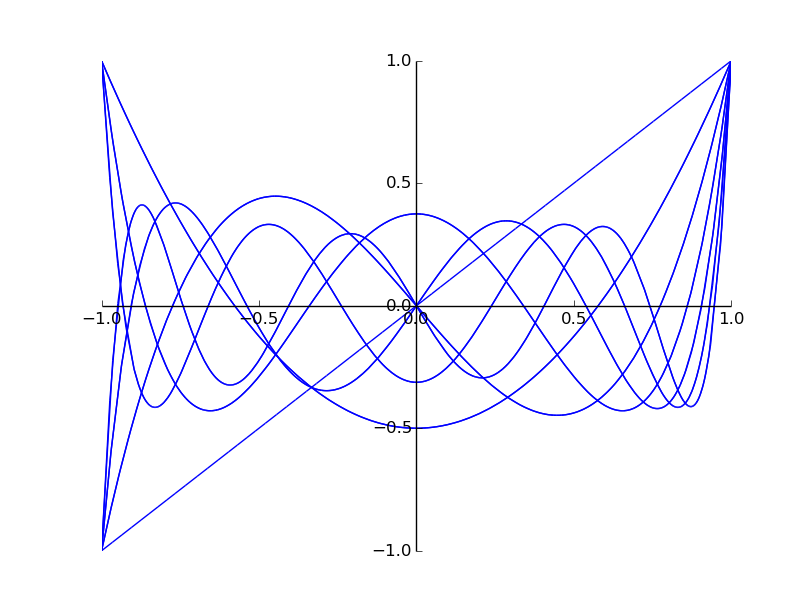
\includegraphics[scale=.25]{imagenes/legendre.png}
\caption{Polinomios de Legendre hasta el orden 8}
\end{center}
\end{figure}



\end{ejemplo}

\section{Teorema fundamental sobre puntos ordinarios}


\begin{definicion} Dada la ecuación diferencial
\[y''(x)+p(x)y'(x)+q(x)y(x)=0\]
donde $p,q$ son funciones   definidas en algún intervalo abierto $I$, diremos que $x_0\in I$ es un \emph{punto ordinario} de la ecuación si $p$ y $q$ son analíticas en $x_0$. Un punto no ordinario se llama \emph{singular}.
\end{definicion}

\begin{ejemplo} En la ecuación del oscilador armónico
\[y''+\omega^2 y=0 \]
todo punto es ordinario.
\end{ejemplo}

\begin{ejemplo} En la ecuación de Legendre
\[(1-x^2)y''-2xy'+p(p+1)y=0 \]
$1$ y $-1$ son puntos singulares, otros valores de $x$ son puntos ordinarios.
\end{ejemplo}

Antes de ir al Teorema más importante de esta sección vamos a enunciar un  lema que nos resultará útil.

\begin{lema}\label{lema:comp_recu}\textbf{Comparación.} Supongamos que tenemos una relación de recurrencia
 \begin{equation}\label{eq:recu2} a_{n}=f_n(a_0,\ldots,a_{n-1})\quad n\geq 2\end{equation}
donde las funciones $f_n$ son crecientes respecto a sus todas las variables. Si la sucesión  $\{a_n\}$ resuelve \eqref{eq:recu2}, la sucesión  $\{b_n\}$ resuelve la desigualdad
 \[b_{n}\leq f_n(b_0,\ldots,b_{n-1})\quad n\geq 2 \]
y además vale que  $b_0\leq a_0$ y $b_1\leq a_1$, entonces $b_n\leq a_n$ para todo $n=2,3,\ldots$. En particular la afirmación se satisface cuando $f_n$ es lineal con coeficientes positivos, es decir $f_n(a_0,\ldots,a_{n-1})=\sum_{k=0}^{n-1}\alpha^n_ka_k$, con $\alpha^n_k\geq 0$ para $k=0,\ldots,n-1$.
\end{lema}
\begin{demo}
Es muy sencilla y la dejamos de ejercicio (evidentemenete hay que utilizar el principio de inducción).
\end{demo}


\begin{teorema}\textbf{Teorema Fundamental Sobre Puntos Ordinarios.}\label{eq:teor_ptos_ord} Sea $x_0$ un punto ordinario de la ecuación
\[y''(x)+p(x)y'(x)+q(x)y(x)=0\]
y sean $a_0,a_1\in\mathbb{R}$. Existe una solución de la ecuación que es analítica en un entorno de $x_0$ y que satisface $y(x_0)=a_0$ e $y'(x_0)=a_1$. El radio de convergencia del desarrollo en serie de $y$ es al menos tan grande como el mínimo de los radios de convergencia de los desarrollos en serie de $p$ y $q$.
\end{teorema}

\begin{demo}
Supongamos, sin perder generalidad, que $x_0=0$. Consideremos que los desarrollos en serie de potencias de $p$ y $q$.
\begin{equation}\label{eq:series_p_q}p(x)=\sum_{n=0}^{\infty}p_nx^n\quad\text{y}\quad q(x)=\sum_{n=0}^{\infty}q_nx^n.
\end{equation}
Supongamos que ambas series convergen en $|x|<R$, para cierto $R>0$. Vamos a aplicar el método de coeficientes indeterminados. Tenemos
\[
    \begin{split}
      y&=\sum_{n=0}^{\infty}a_nx^n=a_0+a_1x+\cdots+a_nx^n+\cdots\\
      y'&=\sum_{n=0}^{\infty}(n+1)a_{n+1}x^n=a_1+2a_2x+\cdots+(n+1)a_{n+1}x^n+\cdots\\
      y''&=\sum_{n=0}^{\infty}(n+1)(n+2)a_{n+2}x^n= 2a_2+2\cdot 3a_3x+\cdots+(n+1)(n+2)a_{n+2}x^n+\cdots.
    \end{split}
\]
Por el  Teorema \ref{teor_oper_series}
\[
   \begin{split}
     q(x)y&=\left(\sum_{n=0}^{\infty}a_nx^n\right)\left(\sum_{n=0}^{\infty}q_nx^n\right)=\sum_{n=0}^{\infty}\left(\sum_{k=0}^na_kq_{n-k}\right)x^n,\\
     p(x)y'&=\left(\sum_{n=0}^{\infty}(n+1)a_{n+1}x^n\right)\left(\sum_{n=0}^{\infty}p_nx^n\right)=\sum_{n=0}^{\infty}\left(\sum_{k=0}^n(k+1)a_{k+1}p_{n-k}\right)x^n.
   \end{split}
\]
Sustituyendo estos, y los anteriores, desarrollos en la ecuación, obtenemos
\[\sum_{n=0}^{\infty}\left\{ (n+1)(n+2)a_{n+2}+ \sum_{k=0}^na_kq_{n-k}+ \sum_{k=0}^n(k+1)a_{k+1}p_{n-k} \right\}x^n.\]
De esta forma deducimos la ecuación de recurrencia que se satisface en una ecuación lineal general de segundo orden en un punto ordinario.
\boxedeq{a_{n+2}=-\frac{ \sum_{k=0}^n\left\{ a_kq_{n-k}+ (k+1)a_{k+1}p_{n-k}\right\}}{n(n+1)}}{eq:rel_recu_gral}
Dados los coeficientes $a_0$ y $a_1$ la relación de recurrencia determina los $a_n$, $n\geq 2$. Queda ver que la serie así definida tiene radio de convergencia al menos $R$.

Tomemos $r$ tal que $0<r<R$. Como las series \eqref{eq:series_p_q} tienen radio de convergencia al menos  $R$,  convergen absolutamente para $x=r$. El criterio de convergencia de series conocido como criterio del resto implica que $p_nr^n,q_nr^n$ son suceciones que tienden a $0$. En particular estan acotadas, y por ello existe $M>0$ tal que
\[ |p_n|r^n,|q_n|r^n\leq M.\]
Tomando módulo en \eqref{eq:rel_recu_gral} y usando las desigualdades de arriba concluímos
\[
  \begin{split}
    |a_{n+2}|&\leq\frac{M}{(n+1)(n+2)r^n} \sum_{k=0}^n\left(|a_k|+ (k+1)|a_{k+1}|\right)r^k\\
&\leq\frac{M}{(n+1)(n+2)r^n} \sum_{k=0}^n\left(|a_k|+ (k+1)|a_{k+1}|\right)r^k+\frac{M|a_{n+1}|r}{(n+1)(n+2)}.
  \end{split}
  \]
En la última desigualdad se agregó un término en apariencia por capricho, pero este término nos servirá para complementar una expresión en el futuro. Definamos la sucesión $b_n$ como la solución de la siguiente relación de recurrencia
\begin{equation}\label{eq:bn_recu}b_{n+2}=\frac{M}{(n+1)(n+2)r^n} \sum_{k=0}^n\left(b_k+ (k+1)b_{k+1}\right)r^k+\frac{Mb_{n+1}r}{(n+1)(n+2)},
\end{equation}
con las condiciones iniciales $b_0=|a_0|$ y $b_1=|a_1|$. Por el Lema \ref{lema:comp_recu} tenemos que $|a_n|\leq b_n$ para todo $n$. Aplicando \eqref{eq:bn_recu} a $n-1$ en lugar de $n$
\begin{equation}\label{eq:bn_recu_2}b_{n+1}=\frac{M}{n(n+1)r^{n-1}} \sum_{k=0}^{n-1}\left(b_k+ (k+1)b_{k+1}\right)r^k+\frac{Mb_{n}r}{n(n+1)},
\end{equation}
Multiplicando  \eqref{eq:bn_recu} por $r$ y usando \ref{eq:bn_recu_2}
\[
\begin{split}
rb_{n+2}=&\frac{M}{(n+1)(n+2)r^{n-1}} \sum_{k=0}^{n-1}\left(b_k+ (k+1)b_{k+1}\right)r^k\\
&+\frac{Mr\left(b_n+ (n+1)b_{n+1}\right)}{(n+1)(n+2)}+\frac{Mb_{n+1}r^2}{(n+1)(n+2)}\\
=&\frac{n(n+1)b_{n+1}-Mb_nr}{(n+1)(n+2)}
+\frac{Mr\left(b_n+ (n+1)b_{n+1}\right)}{(n+1)(n+2)}\\
&+\frac{Mb_{n+1}r^2}{(n+1)(n+2)}\\
=&\frac{(n(n+1)+Mr(n+1)+Mr^2)}{(n+1)(n+2)}b_{n+1},
\end{split}
\]
Entonces
\[\lim_{n\to\infty}\frac{|b_{n+2}x^{n+2}|}{|b_{n+1}x^{n+1}|}=\lim_{n\to\infty}\frac{(n(n+1)+Mr(n+1)+Mr^2)}{(n+1)(n+2)}\frac{|x|}{r}=\frac{|x|}{r}.
\]
Luego la serie $\sum_{n=0}^{\infty}b_nx^n$ converge para $|x|<r$. Como $|a_n|\leq b_n$ la misma afirmación es cierta para $\sum_{n=0}^{\infty}a_nx^n$. Como $r<R$ fue elegido arbitrariamente, tenemos que $\sum_{n=0}^{\infty}a_nx^n$ converge en $|x|<R$.
\end{demo}


\section{Puntos singulares, método de Frobenius}

\subsection{Series de Frobenius}
\begin{definicion}\textbf{ Sigularidades, Polos.} Sea $f$ definida en un intervalo abierto $I$ con valores en $\rr$. Diremos que $f$ posee un \emph{polo de orden $k$} en $x_0\in\rr$, si la función $(x-x_0)^kf(x)$ es analítica en un entorno de $x_0$. Vale decir que $(x-x_0)^kf(x)$ se desarrolla en serie de potencias.
\[(x-x_0)^kf(x)=\sum_{n=0}^{\infty}a_n(x-x_0)^n.\]
En consecuencia
\[f(x)=\sum_{n=0}^{\infty}a_n(x-x_0)^{n-k}=\frac{a_0}{(x-x_0)^k}+\cdots+\frac{a_{k-1}}{(x-x_0)}+a_k+a_{k+1}(x-x_0)+\cdots.\]
Este tipo de desarrollo en serie es un caso particular de serie de Laurent.

Cuando el orden de un polo es $1$ se lo denomina \emph{polo simple}.
\end{definicion}



\begin{definicion} Un punto singular $x_0$ de la ecuación
\[y''(x)+p(x)y'(x)+q(x)y(x)=0\]
se llama singular regular si $p(x)$ tiene un polo a lo sumo simple en $x_0$ y $q(x)$ tiene un polo a lo sumo de orden $2$ en $x_0$. Es decir
\[(x-x_0)p(x)\quad\hbox{y}\quad (x-x_0)^2q(x)\]
son analíticas en $x_0$.
\end{definicion}
Algunas de las ecuaciones más importantes de la Física-Matemática tienen puntos singulares regulares.

\begin{ejemplo} 1 y -1 son puntos singulares regulares de la ecuación de Legendre de orden $p$
\[y''-\frac{2x}{1-x^2}y'+\frac{p(p+1)}{1-x^2}y=0\]
\end{ejemplo}


\begin{ejemplo} 0 es un punto singular regular de la ecuación de Bessel de orden $p$
\[y''+\frac{1}{x}y'+\left(1-\frac{p^2}{x^2}\right)y=0\]
\end{ejemplo}

El método de coeficientes indeterminados puede fallar en los puntos donde $p$ y $q$ tienen polos. En su lugar vamos a proponer otro tipo de desarrollo en serie. Lo vamos a motivar con un ejemplo.

\begin{ejemplo} Consideremos la ecuación de Euler, para $p,q\in\rr$
\[y''+\frac{p}{x}y'+\frac{q}{x^2}y=0\]
o equivalentemente
\[x^2y''+pxy'+qy=0\]
Aquí es facil verificar que las funciones
\[P(x):=\frac{p}{x}\quad\hbox{ y }\quad Q(x):= \frac{q}{x^2}\]
satisfacen que
\[\frac{Q'+2PQ}{Q^{\frac{3}{2}}}\quad\text{es constante.}\]
 Cuando se daba esta condición, el ejercicio 6 de la página 102 del libro de Simmons nos enseña que podemos reducir la ecuación a una ecuación con coeficientes constantes por medio del cambio de la variable independiente
\[z=\int\sqrt{Q}dx\]
En este caso, obviando las constantes, el cambio de variables que debemos hacer es
\[z=\ln(x)\]
Aquí  asumimos $x>0$. Seguramente, a esta altura del curso,  el alumno ya hizo los cálculos que muestran que la ecuación de Euler se transforma,  por medio del cambio de variables propuesto, en la ecuación a coeficientes constantes
\[y''+(p-1)y'+qy=0.\]
Cuya ecuación característica es
\[\lambda^2+(p-1)\lambda+q=0\]
Resolviendo esta ecuación con SymPy

\begin{lstlisting}
s,p,q=symbols('s,p,q')
Raices=solve(s**2+(p-1)*s+q,s)
Raices[0]
-p/2 - sqrt(p**2 - 2*p - 4*q + 1)/2 + 1/2
Raices[1]
-p/2 + sqrt(p**2 - 2*p - 4*q + 1)/2 + 1/2
\end{lstlisting}
Obtenemos las raíces
\[s_1= -\frac{p-1}{2} - \frac{\sqrt{p^2 - 2p - 4q + 1}}{2}   \quad\text{y}\quad s_2=-\frac{p-1}{2} +\frac{\sqrt{p^2 - 2p - 4q + 1}}{2} .\]
 Si $s_1\neq s_2$ dos soluciones linealmente independientes son:
\[y_1(z)=e^{s_1z}\quad\hbox{y}\quad y_2(z)=e^{s_2z}\]
 Si $s_1=s_2$
\[y_1(z)=e^{s_1z} \quad\hbox{y}\quad y_2(z)=ze^{s_1z}\]
son soluciones linealmente independientes. Asumamos que las raices $s_1$ y $s_2$ son reales, entonces como $z=\ln(x)$, las soluciones en términos de la variable $x$ son
\[y_1(x)=x^{s_1}\quad\hbox{y}\quad y_2(x)=x^{s_2}\quad\text{para }  s_1\neq s_2\]
y
\[y_1(x)=x^{s_1} \quad\hbox{y}\quad y_2(x)=\ln(x)x^{s_1}\quad\text{para }  s_1= s_2\]



Estas funciones, a menos que $s_1$ y $s_2$ sean enteros positivos, ya no son analíticas en cero, pues una función analítica es derivable infinitas veces y claramente hay derivadas (o las mismas funciones si las raices son negativas) de $y_1$ e $y_2$ que son discontinuas.
\end{ejemplo}


De modo que, como era de suponer, no podremos encontrar en general en un punto singular una solución analítica.  Vamos a intentar flexibilizar nuestro método para incluir otro tipo de desarrollo en serie, que está inspirado en los resultados obtenidos para la ecuación de Euler.

\begin{definicion} A una expresión de la forma
 \[y(x)=(x-x_0)^m(a_0+a_1(x-x_0)+a_2(x-x_0)^2+\cdots),\]
donde $m\in\rr$ y $a_0\neq 0$, lo llamaremos \emph{Serie de Frobenius}.
\end{definicion}
Las series de Frobenius no son series de potencias ni de Laurent ya que en ellas aparecen potencias no enteras.

El método de Frobenius consiste en proponer como solución de una ecuación diferencial una serie de Frobenius. Este método tiene éxito, por ejemplo, en los puntos sigulares regulares de ecuaciones diferenciales lineales de segundo orden.

\begin{ejemplo} En este ejemplo ilustramos el método de Frobenius. Consideremos la ecuación
\begin{equation}\label{eq:ejem_sim}y''+\left(\frac{1}{2x}+1\right)y'-\left(\frac{1}{2x^2}\right)y=0.
\end{equation}
Notar que $x=0$ es regular singular. Desarrollaremos el método de Frobenius, primero ``a mano'' y por último con SymPy.

Proponemos como solución

 \[y(x)=x^m\sum_{n=0}^{\infty}a_{n}x^n=\sum_{n=0}^{\infty}a_{n}x^{n+m}\]
y calculamos
\[
    \begin{split}
     -\frac{1}{2x^2}y&=-\sum_{n=0}^{\infty}\frac{a_n}{2}x^{m+n-2}=-\frac{a_0}{2}x^{m-2}
-\frac{a_1}{2}x^{m-1}-\cdots-\frac{a_{n+2}}{2}x^{m+n}-\cdots\\
      y'&=\sum_{n=0}^{\infty}(m+n)a_{n}x^{m+n-1}=ma_0x^{m-1}+(m+1)a_1x^m+\cdots+(m+n+1)a_{n+1}x^{m+n}+\cdots\\
      \frac{1}{2x}y'&=\sum_{n=0}^{\infty}\frac{(m+n)a_{n}}{2}x^{m+n-2}=\frac{ma_0}{2}x^{m-2}+\frac{(m+1)a_1}{2}x^{m-1}+\cdots+\frac{(m+n+2)a_{n+2}}{2}x^{m+n}+\cdots\\
      y''&=\sum_{n=0}^{\infty}(m+n)(m+n-1)a_{n}x^{m+n-2}\\
&= m(m-1)a_0x^{m-2}+(m+1)ma_1x^{m-1}+\cdots+(m+n+2)(m+n+1)a_{n+2}x^{m+n}+\cdots.
    \end{split}
\]
Sumando las cuatro igualdades miembro a miembro y sustiyendo en \eqref{eq:ejem_sim}

\[
  \begin{split}
    0=& \left(-\frac{1}{2} +\frac{m}{2}+m(m-1)\right)a_0x^{m-2}  + \left(-\frac{a_1}{2}+ma_0+\frac{(m+1)a_1}{2}+ (m+1)ma_1 \right)x^{m-1}+\cdots \\
  &+\left( -\frac{a_{n+2}}{2}+(m+n+1)a_{n+1}+ \frac{(m+n+2)a_{n+2}}{2}+(m+n+2)(m+n+1)a_{n+2} \right)x^{m+n}+\cdots\\
 =&\frac12\left(2m+1\right)(m-1) a_0x^{m-2}+ \frac{1}{2} \, {\left( 2 \, a_{0} + (1+2(m+1))\, a_{1}\right)}m x^{m-1}+\cdots\\
 &+\frac12\left(   2a_{n+1}+ (2(m+n+2)+1)a_{n+2}  \right)(m+n+1)x^{m+n}+\cdots.
  \end{split}
\]
Igualando a cero los coeficientes de cada exponente obtenemos las ecuaciones

\begin{equation}\label{eq:ecua_ejem_frob}
    \begin{split}
      \frac12\left(2m+1\right)(m-1) a_0&=0\\
       \frac{1}{2}  \left(   2 a_{0} + (1+2(m+1)) a_{1}\right)m&=0\\
                                      &\vdots\\
     \left(   2a_{n+1}+ (2(m+n+2)+1)a_{n+2}  \right)(m+n+1) &=0\\
    \end{split}
\end{equation}
Despejando de la última ecuación nos queda la relación de recurrencia de un término
\boxedeq{a_{n+2}=-\frac{2a_{n+1}}{2(m+n+2)+1}.}{eq:recu_ecua_ejem_frob}
Para llegar a esta igualdad debimos suponer $2(m+n+2)+1\neq 0$.
La primera de las ecuaciones en \eqref{eq:ecua_ejem_frob} es importante puesto que determina el valor de $m$. Se llama ecuación indicial. Vemos que si tomamos $m=1$ o $m=-1/2$ se resuelve la primera ecuacion. Supongamos $m=1$. Entonces \eqref{eq:recu_ecua_ejem_frob} se transforma en
\[
a_{n+2}=-\frac{2a_{n+1}}{2n+7},\quad n=-1,0,\ldots.
\]
Con ayuda de la relación de recurrencia podemos determinar el radio de convergencia de la serie sin necesidad de conocer el valor de los $a_n$

\[\lim_{n\to\infty}\frac{|a_{n+1}x^{n+1}|}{|a_{n}x^{n}|}=
\lim_{n\to\infty}\frac{2|x|}{2n+7}=0.\]
Por consiguiente el radio de convergencia es infinito.  Iterando la relación de recurrencia llegamos
\[a_{n}=-\frac{2}{2n+3}a_{n-1}=\frac{2}{(2n+3)(2n+1)}a_{n-2}=\cdots=
\frac{(-1)^n2^{n}}{(2n+3)(2n+1)\cdots 5}a_0.\]
El valor de $a_0$ determina al resto de los $a_n$ y se puede elegir arbitrariamente. Supongamos que $a_0=1$. Hemos hallado la siguiente solución
\boxedeq{y_1(x)=x\sum_{n=0}^{\infty}(-1)^n\frac{2^{n}}{(2n+3)(2n+1)\cdots 5}x^n.}{}
Cuando $m=-\frac12$, la relación de recurrencia es
\[a_{n+1}=-\frac{a_{n}}{n+1}.\]
Por ende
\[a_n=-\frac{a_{n-1}}{n}=\frac{1}{n(n-1)}a_{n-2}=\cdots=\frac{(-1)^n}{n!}a_{0}=\frac{(-1)^n}{n!}.\]
Conseguimos la solución
\boxedeq{y_2(x)=x^{-\frac12}\sum_{n=0}^{\infty}\frac{(-1)^n}{n!}x^n=\frac{e^{-x}}{\sqrt{x}}}{}
Estas dos soluciones son linealmente independientes. Para justificar esta afirmación basta ver que $y_1(0)=0$ y $\lim_{x\to 0+}y_2(x)=+\infty$. Estas igualdades hacen imposible la relación $c_1y_1+c_2y_2=0$ a menos que $c_1=c_2=0$.

Resolvamos el ejemplo con SymPy.

\begin{lstlisting}
orden=5
a=symbols('a0:%s' %orden)
x,m=symbols('x,m')
y=x**m*sum([a[i]*x**i for i in range(orden)])
Ecua=y.diff(x,2)+(1/(2*x)+1)*y.diff(x,1)-(1/(2*x**2))*y
#Dividimos por m-2 asi todos los exponentes son enteros positivos
Ecua=Ecua/x**(m-2)
Ecua=Ecua.expand()
Ecuaciones=[Ecua.diff(x,i).subs(x,0)/factorial(i) for i in range(orden)]
for ec in Ecuaciones:
...     ec
...
a0*m**2 - a0*m/2 - a0/2
a0*m + a1*m**2 + 3*a1*m/2
a1*m + a1 + a2*m**2 + 7*a2*m/2 + 5*a2/2
a2*m + 2*a2 + a3*m**2 + 11*a3*m/2 + 7*a3
a3*m + 3*a3 + a4*m**2 + 15*a4*m/2 + 27*a4/2

\end{lstlisting}

Con esta parte del script hemos generado la lista de las 5 primeras ecuaciones.
Resolvamos la ecuación indicial

\begin{lstlisting}
Sol_Ecua_Ind=solve(Ecuaciones[0],m)
Sol_Ecua_Ind
[-1/2, 1]
\end{lstlisting}

Sustituyamos los valores de $m$ en la lista de ecuaciones, agreguemos la ecuación $a_0=1$, resolvamos para los $a_i$ y sustituyamos la solución en $y$. Obtenemos la primer solución (truncada)
\begin{lstlisting}
Ecuaciones1=[ec.subs(m,Sol_Ecua_Ind[1]) for ec in Ecuaciones]
Ecuaciones1
[0, a0 + 5*a1/2, 2*a1 + 7*a2, 3*a2 + 27*a3/2, 4*a3 + 22*a4]
Ecuaciones1[0]=a[0]-1
Ecuaciones1
[a0 - 1, a0 + 5*a1/2, 2*a1 + 7*a2, 3*a2 + 27*a3/2, 4*a3 + 22*a4]
sol=solve(Ecuaciones1,a)
y1=y.subs(sol).subs(m,Sol_Ecua_Ind[1])
y1
x*(16*x**4/3465 - 8*x**3/315 + 4*x**2/35 - 2*x/5 + 1)


\end{lstlisting}
La segunda solución se obtinene
\begin{lstlisting}
Ecuaciones2=[ec.subs(m,Sol_Ecua_Ind[0]) for ec in Ecuaciones]
Ecuaciones2
[0, -a0/2 - a1/2, a1/2 + a2, 3*a2/2 + 9*a3/2, 5*a3/2 + 10*a4]
Ecuaciones2[0]=a[0]-1
sol=solve(Ecuaciones2,a)
y2=y.subs(sol).subs(m,Sol_Ecua_Ind[0])
(x**4/24 - x**3/6 + x**2/2 - x + 1)/sqrt(x)

\end{lstlisting}



\end{ejemplo}

\subsection{Ecuación de Bessel, funciones de Bessel de primera especie}\label{sec:bessel_1}

\subsubsection{Relaciones de recurrencia y solución por el método de Frobenius}

\begin{definicion} Recordemos a la ecuación de Bessel de orden $p$ ($p>0$)
 \[y''+\frac{1}{x}y'+\left(1-\frac{p^2}{x^2}\right)y=0\]
\end{definicion}

En $x=0$ la ecuación de Bessel tiene un punto  singular regular. Vamos a aplicarle el método de Frobenius. Trabajeremos exclusivamente con SymPy.

\begin{lstlisting}
orden=8
a,x,m,p=symbols(['a0:%s' %orden, 'x','m','p'] )
y=x**m*sum([a[i]*x**i for i in range(orden)])
EDif=y.diff(x,2)+1/x*y.diff(x,1)+(1-p**2/x**2)*y
EDif=(EDif/x**(m-2)).simplify()
ECoef=[EDif.diff(x,i).subs(x,0)/factorial(i) for i in range(orden)]
SolEInd=solve(ECoef[0],m)
\end{lstlisting}

Las raíces de la ecuación indicial son
\boxedeq{m=p\quad\text{y}\quad m=-p}{eq:sol_ec_ind}
Vamos a trabajar con la raíz $m=p$.

\begin{lstlisting}
ECoefA=[ec.subs(m,Sol_Ecua_Ind[1]) for ec in ECoef]
for ec in ECoefA:
...     pprint(ec)

\end{lstlisting}

\[
\begin{split}
 0 & = 0\\
0&=2 a_{1} p + a_{1}\\
0&=a_{0} + 4 a_{2} p + 4 a_{2}\\
0&=a_{1} + 6 a_{3} p + 9 a_{3}\\
0&=a_{2} + 8 a_{4} p + 16 a_{4}\\
0&=a_{3} + 10 a_{5} p + 25 a_{5}\\
0&=a_{4} + 12 a_{6} p + 36 a_{6}\\
0&=a_{5} + 14 a_{7} p + 49 a_{7}\\
\end{split}
\]



Se puede observar que estas ecuaciones relacionan  $a_n$ con $a_{n-2}$, i.e. que son relaciones de dos términos.  Podemos hacer explícita la relación

\begin{lstlisting}
for i in range(1,orden):
    iter=solve(ECoefA[i],a[i])[0].factor()
    print str(a[i])+'='+str(iter)
a1=0
a2=-a0/(4*(p + 1))
a3=-a1/(3*(2*p + 3))
a4=-a2/(8*(p + 2))
a5=-a3/(5*(2*p + 5))
a6=-a4/(12*(p + 3))
a7=-a5/(7*(2*p + 7))
\end{lstlisting}

 La ecuación $a_1(2p+1)=0$ no fue correctamente resuelta por SymPy. SymPy consigna la solución $a_1=0$, pero si  $p=-1/2$ cualquier $a_1$ es solución. Este caso lo estudiaremos separadamente después, por ahora supondremos $p\neq -1/2$. Luego la primera ecuación implica que $a_1=0$ y por consiguiente, puesto que todo $a_n$, con $n$ impar, se relaciona con $a_1$ vamos a tener que $a_n=0$ cuando $n$ es impar. Más abajo veremos que SymPy confirma esta aseveración. Ahora resolvamos las ecuaciones, en el sentido de expresar todos los coeficientes en función de $a_0$. No pedimos que nos resuelva la ecuación para $a_0$, pues, como dijimos, $a_0$ es arbitrario.


\begin{lstlisting}
sol=solve(ECoefA,a[1:])
for i in sol:
...     print str(i)+'='+str(sol[i].factor())
...
a1=0
a5=0
a7=0
a2=-a0/(4*(p + 1))
a6=-a0/(384*(p + 1)*(p + 2)*(p + 3))
a3=0
a4=a0/(32*(p + 1)*(p + 2))

\end{lstlisting}
No queda muy claro cual es la ley que siguen los números 4, 32, 384, etc. que aparecen en el denominador. De modo que nos asitiremos ``manualmente'' a partir de la relación de recurrencia que es
\boxedeq{a_{2n}=-\frac{1}{4n(p+n)}a_{2n-2}}{eq:recu_bessel}
Iterando esta relación
\[
\begin{split}
  a_{2n}&=-\frac{1}{4n(p+n)}a_{2n-2}\\
       &=\frac{1}{4n(p+n-1)}\cdot\frac{1}{4(n-1)(p+n-1)}a_{2n-4}=\cdots\\
       & =(-1)^n\frac{1}{4^nn!(p+n)(p+n-1)\cdots (p+1)}a_{0}.
\end{split}
\]
Obtenemos la solución
\boxedeq{y(x)=x^p\sum_{n=0}^{\infty}\frac{(-1)^na_0}{4^nn!(p+n)(p+n-1)\cdots (p+1)}x^{2n}}{eq:sol_bessel_1}
Más adelante veremos que cierta elección especial de $a_0$ no lleva a lo que denominaremos funciones de Bessel.
\begin{lstlisting}
y.subs(sol)
\end{lstlisting}

\[
x^{m} \left(- \frac{a_{0} x^{6}}{384 \left(p + 1\right) \left(p + 2\right) \left(p + 3\right)} + \frac{a_{0} x^{4}}{32 \left(p + 1\right) \left(p + 2\right)
} - \frac{a_{0} x^{2}}{4 p + 4} + a_{0}\right),
\]
el output confirma \eqref{eq:sol_bessel_1}.

\subsubsection{Función Gamma y la función de Bessel de primera especie}

Nuestro obtjetivo es encontrar dos soluciones linealmente independientes de la ecuación de Bessel. Hemos encontrado una que corresponde a la solución de la ecuación de índices $m=p$, la otra surgirá de la solución $m=-p$. Pero aún nos restaría elegir el valor de $a_0$. El criterio que utilizaremos para elegirlo será que nos simplifique lo más posible la expresión  \eqref{eq:sol_bessel_1}. Si $p$ fuese un entero positivo, eligiendo $a_0$ como $1/2^pp!$ la expresión quedaría
\[y(x)=\sum_{n=0}^{\infty}\frac{(-1)^n}{n!(p+n)!}\left(\frac{x}{2}\right)^{2n+p}\]
No obstante, nos previene utilizar este $a_0$ el hecho de que $p$ podría no ser entero, y en ese caso no es claro que significa $p!$. El propósito de esta subsección es introducir una extensión de la función factorial a una función de variable real.

\begin{definicion}\label{def:gamma} Para $p>0$ definimos la \emph{función Gamma} por
\begin{equation}\label{eq:gamma}\Gamma(p):=\int_0^{\infty}t^{p-1}e^{-t}dt
\end{equation}
\end{definicion}

En la clase demostraremos que la integral impropia en la definición converge. Además demostraremos las siguientes relaciones
\boxedeq{\begin{split}\Gamma(1)&=1\\
 \Gamma(p+1)&=p\Gamma(p)\end{split}}{eq:recu_gamma}
Estas igualdades  implican, cuando $p=n$ es entero positivo, que $\Gamma(n+1)=n\Gamma(n)=\cdots=n!\Gamma(1)=n!$. Luego podemos ver a la función gamma como una extensión de la función factorial a los reales no negativos. Notar que
\[\lim_{p\to 0+}\Gamma(p)=\lim_{p\to 0+}\frac{\Gamma(p+1)}{p}=+\infty.\]
La función Gamma tiende a  infinito cuando nos acercamos a cero por derecha.

La Definición \ref{eq:gamma} es válida para $p>0$. Utilizando la relación \eqref{eq:recu_gamma} podemos extender la función a $p<0$. Concretamente,  supongamos  que $-1<p<0$, en  este caso definimos
\boxedeq{\Gamma(p):=\frac{\Gamma(p+1)}{p}.}{eq:gama_iter}
Observar que el segundo miembro esta bien definido pues $p+1>0$. Como consecuencia de esta definición tendremos
\[\lim_{p\to 0-}\Gamma(p)=\lim_{p\to 0-}\frac{\Gamma(p+1)}{p}=-\infty.\]
y
\[\lim_{p\to -1+}\Gamma(p)=\lim_{p\to -1+}\frac{\Gamma(p+1)}{p}=-\infty.\]
Ahora podemos extender $\Gamma$ a $p\in (-2,1)$. Pues  podemos usar la fórmula \eqref{eq:gama_iter} y el hecho de que ya tenemos definida la función Gamma en $(-1,0)$. Continuando de esta forma, definimos $\Gamma$ para cualquier valor de $p<0$ y $p\notin \mathbb{Z}$. Si $n$ es un entero negativo ocurre que
\[\lim_{p\to n+}\Gamma(p)=(-1)^n\infty\quad\text{y}\quad \lim_{p\to n-}\Gamma(p)=(-1)^{n-1}\infty.\]




\begin{figure}[h]
\begin{center}
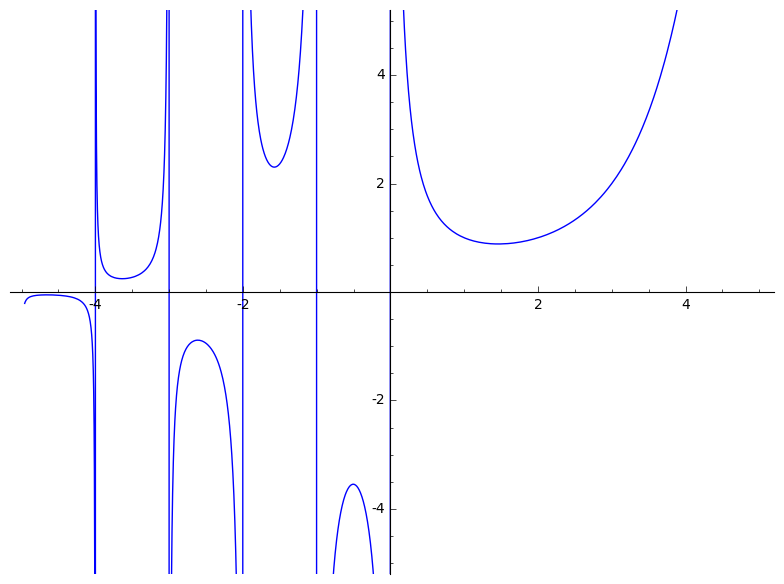
\includegraphics[scale=.4]{imagenes/gamma.png}
\caption{La función gamma $\Gamma$}
\end{center}
\end{figure}
Ahora estamos en condiciones de definir la función de Bessel de primera espacie que resulta de tomar $a_0$ como $1/2^p\Gamma(p+1)$.

\begin{definicion}\label{def:bessel_primera} Definimos la función de Bessel de primera especie como
\[J_p(x)=\sum_{n=0}^{\infty}\frac{(-1)^n}{n!\Gamma(p+n+1)}\left(\frac{x}{2}\right)^{2n+p}\]
\end{definicion}


Una aproximación a esta función se programa en SymPy de manera muy sencilla. Una vez definida esta función podemos aprovecharla  para graficar varias funciones de Bessel de distintos órdenes.

\begin{lstlisting}
p,x=symbols('p,x')
J= sum([(-1)**n/factorial(n)/gamma(p+n+1)*(x/2)**(2*n+p) for n in range(30)])
p1=plot(J.subs(p,1),(x,0,20),line_color=(1,0,0))
p2=plot(J.subs(p,2),(x,0,20),line_color=(0,1,0))[0]
p1.append(p2)
p2=plot(J.subs(p,3),(x,0,20),line_color=(0,0,1))[0]
p1.append(p2)
p1.show()
\end{lstlisting}
\begin{figure}[h]
\begin{center}
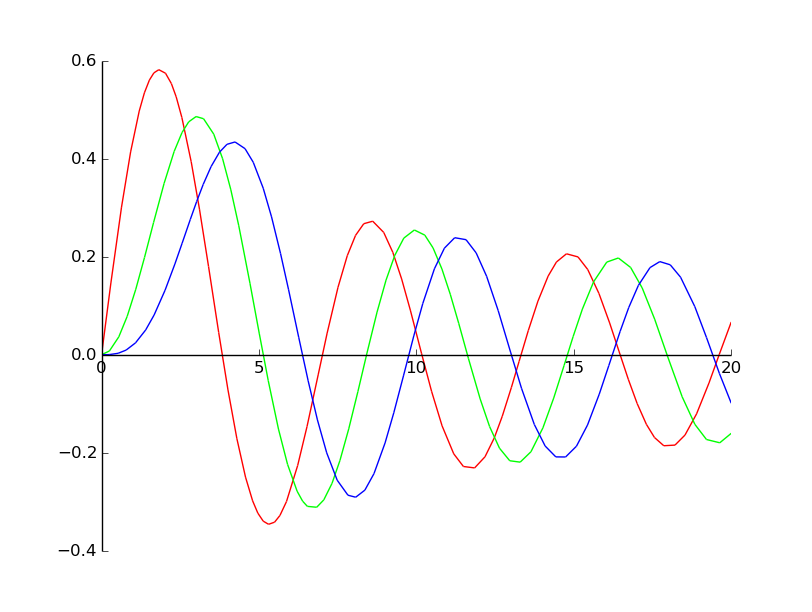
\includegraphics[scale=.5]{imagenes/bessel.png}
\end{center}

\caption{Funciones de Bessel $J_p$, $p=1,2,3$}\label{fig:bessel}

\end{figure}





Ahora consideremos la solución $m=-p$ de la ecuación indicial.
\begin{lstlisting}
ECoefB=[ec.subs(m,Sol_Ecua_Ind[0]) for ec in ECoef]
for i in range(1,orden):
    iter=solve(ECoefB[i],a[i])[0].factor()
    print str(a[i])+'='+str(iter)

a1=0
a2=a0/(4*(p - 1))
a3=a1/(3*(2*p - 3))
a4=a2/(8*(p - 2))
a5=a3/(5*(2*p - 5))
a6=a4/(12*(p - 3))
a7=a5/(7*(2*p - 7))

\end{lstlisting}
Estas relaciones siguen el mismo patrón que la relación de recurrencia \eqref{eq:recu_bessel} con $-p$ en lugar de $p$. No obstante, la situación para la raíz $-p$ no es exactamente igual a la de la raíz $p$. La diferencia radica en que cuando $p\in\frac12\mathbb{N}=\frac12,1,\frac32,\ldots$  la expresión en el denominador en la relación
\boxedeq{a_{n}=\frac{a_{n-2}}{n(2p-n)}}{eq:rel_recu_bess-p}
se puede anular y esto  impediría que pasasemos de miembro esta expresión como hicimos. Notar que este problema ocurre cuando la diferencia de las dos raíces $p-(-p)=2p$ es un entero positivo.  Esto último lo remarcamos porque veremos más adelante que en general es un problema que la diferencia de las raíces de la ecuación indicial sean negativas. También $p=0$ es una situación problemática, dado que en este caso $p=-p$ y por consiguiente no estamos en condiciones de encontrar una solución linealmente independiente de $J_0$. En síntesis $p=0,\frac12,1,\frac32,\ldots$ son valores problemáticos para $p$.

Cuando $p$ no es uno de los valores problemáticos, estamos en condiciones de definir
\begin{definicion}\label{def:bessel_segunda} Definimos la función de Bessel de primera especie $J_{-p}$ ($p\notin\frac12\mathbb{N}$) como
\[J_{-p}(x)=\sum_{n=0}^{\infty}\frac{(-1)^n}{n!\Gamma(-p+n+1)}\left(\frac{x}{2}\right)^{2n-p}\]
\end{definicion}
Grafiquemos algunas de estas funciones de Bessel, la función de Bessel $J$ que habíamos introducido en SymPy arriba, sigue siendo útil.
\begin{lstlisting}
p1=plot(J.subs(p,-1.0/3),(x,0,20),line_color=(1,0,0),ylim=(-2,2))
p2=plot(J.subs(p,-2.0/3),(x,0,20),line_color=(0,1,0),ylim=(-2,2))
p3=plot(J.subs(p,-5.0/3),(x,0,20),line_color=(0,0,1),ylim=(-2,2))
p1.append(p3[0])
p1.append(p3[0])
\end{lstlisting}

\begin{figure}[h]
\begin{center}
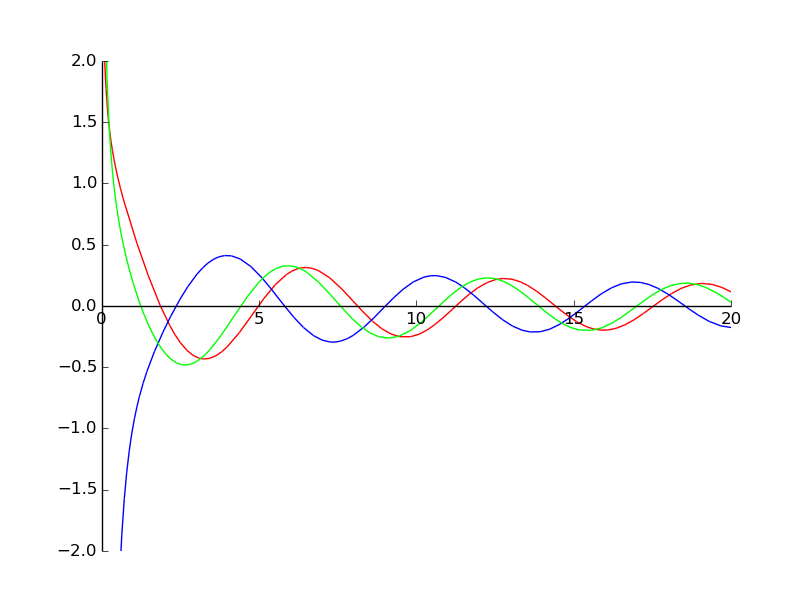
\includegraphics[scale=.5]{imagenes/bessel2.png}
\end{center}
\caption{Funciones de Bessel $J_{-1/3}$, $J_{-2/3}$ y $J_{-5/3}$.}
\end{figure}
Más adelante vamos a seguir estudiando con más profundidad la ecuación de Bessel.

\subsection{Teorema fundamental sobre puntos singulares regulares}\label{eq:sec_teor_fund_frob}
Habiendo visto algunos ejemplos, ahora pasaremos a discutir la situación general del método de Frobenius.

Supongamos $x=0$ un punto regular singular de la ecuación
\begin{equation}\label{eq:dif_2_orden} y''+p(x)y'+q(x)y=0.
\end{equation}
Supongamos que $xp(x)$ y $x^2q(x)$ poseen los  siguientes desarrollos en serie
\[xp(x)=\sum_{n=0}^{\infty}p_nx^n\quad\text{y}\quad x^2q(x)=\sum_{n=0}^{\infty}q_nx^n\]
Proponemos como solución
\[y=x^{m}\sum_{n=0}^{\infty}a_nx^n=\sum_{n=0}^{\infty}a_nx^{m+n}.\]
Empecemos por hallar las relaciones de recurrencia para los coeficientes $a_n$, $n=0,1,\ldots$.   Tenemos
\begin{subequations}
    \begin{align}
      y'&=\sum_{n=0}^{\infty}(m+n)a_{n}x^{m+n-1}\\
      y''&=\sum_{n=0}^{\infty}(m+n)(m+n-1)a_{n}x^{m+n-2}\notag\\
&=x^{m-2}\sum_{n=0}^{\infty}(m+n)(m+n-1)a_{n}x^{n}\label{eq:der_seg} .
    \end{align}
  \end{subequations}
Luego

\begin{equation}\label{eq:der_pri}
  \begin{split}
    p(x)y'(x)&=\frac{1}{x}\left(\sum_{n=0}^{\infty}p_nx^n\right)\left(\sum_{n=0}^{\infty}(m+n)a_{n}x^{m+n-1}\right)\\
&=x^{m-2}\left(\sum_{n=0}^{\infty}p_nx^n\right)\left(\sum_{n=0}^{\infty}(m+n)a_{n}x^{n}\right)\\
&= x^{m-2}\sum_{n=0}^{\infty}\left(\sum_{k=0}^np_{n-k}(m+k)a_k\right)x^n\\
&= x^{m-2}\sum_{n=0}^{\infty}\left(\sum_{k=0}^{n-1}p_{n-k}(m+k)a_k+p_0(m+n)a_n\right)x^n
  \end{split}
\end{equation}
Ahora desarrollemos $q(x)y(x)$,
\begin{equation}\label{eq:der_cero}
  \begin{split}
    q(x)y(x)&=\frac{1}{x^2}\left(\sum_{n=0}^{\infty}q_nx^n\right)\left(\sum_{n=0}^{\infty}a_{n}x^{m+n}\right)\\
&=x^{m-2}\left(\sum_{n=0}^{\infty}q_nx^n\right)\left(\sum_{n=0}^{\infty}a_{n}x^{n}\right)\\
&= x^{m-2}\sum_{n=0}^{\infty}\left(\sum_{k=0}^nq_{n-k}a_k\right)x^n\\
&= x^{m-2}\sum_{n=0}^{\infty}\left(\sum_{k=0}^{n-1}q_{n-k}a_k+q_0a_n\right)x^n
  \end{split}
\end{equation}
A partir de \eqref{eq:dif_2_orden}, \eqref{eq:der_cero},\eqref{eq:der_pri} y \eqref{eq:der_seg} obtenemos
\begin{equation}
\begin{split}
  0=&x^{m-2}\sum_{n=0}^{\infty}\bigg\{\left[(m+n)(m+n-1)+p_0(m+n)  +q_0  \right] a_{n}\\&+\sum_{k=0}^{n-1}a_k\left[p_{n-k}(m+k) +
q_{n-k}\right]\bigg\}x^n.
\end{split}
\end{equation}
Entonces se debe satisfacer
\boxedeq{\left[(m+n)(m+n-1)+p_0(m+n)  +q_0  \right] a_{n}+\sum_{k=0}^{n-1}a_k\left[p_{n-k}(m+k) +
q_{n-k}\right]=0,}{eq:recu_gral_frob}
para $n=0,1,\ldots$. Definamos
\boxedeq{f(m)=m(m-1)+p_0m+q_0.}{eq:func_f}
Entonces las ecuaciones \eqref{eq:recu_gral_frob} se escriben
\boxedeq{f(m+n)a_n=-\sum_{k=0}^{n-1}a_k\left[p_{n-k}(m+k) +
q_{n-k}\right],\quad n=0,1,\ldots}{eq:recu_gral_frob_2}
La primera de estas ecuaciones es
\begin{definicion} Definimos la  ecuación indicial por
\begin{equation}\label{eq:eq_indicial}
  f(m)=m(m-1)+p_0m+q_0=0.
\end{equation}

\end{definicion}

Si $m$ resuelve la ecuación indicial entonces $m$ resuelve la ecuación \eqref{eq:recu_gral_frob_2} para $n=0$ y el valor de $a_0$ se puede elegir arbitrariamente.

Supongamos que la ecuación indicial tiene las soluciones $m_2\leq m_1$. Podría ocurrir que las soluciones fueran complejos conjugados, pero no trataremos este caso aquí. Ahora discutamos cuando es posible resolver las relaciones de recurrencia \eqref{eq:recu_gral_frob_2}. El único problema que podría ocurrir es que  $f(m+n)=0$ para algún valor de $n=1,2,\ldots$, dado que en ese caso \eqref{eq:recu_gral_frob_2} se reduce a
\begin{equation}\label{eq:ec_enter} 0=-\sum_{k=0}^{n-1}a_k\left[p_{n-k}(m+k) +
q_{n-k}\right].
\end{equation}
Esta ecuación no nos dice nada sobre $a_n$ y no podemos esperar que se satisfaga. Sin embargo, cuando $m=m_1$ esta desafortunada situación no se da, de lo contrario  $m_1+n$ sería una raíz de la ecuación indicial distinta que $m_2$ y $m_1$. En consecuencia, \emph{si $m=m_1$ y $a_0\neq 0$ es elegido arbitrariamente las ecuaciones \eqref{eq:recu_gral_frob_2} determinan los coeficientes $a_n$, $n=1,2,\ldots$.}

Cuando $m=m_2$ si puede ocurrir que $f(m_2+n)=0$, esto es así cuando $m_2+n=m_1$ para algún $n=1,2,\ldots$, vale decir cuando $m_1-m_2\in\mathbb{Z}$.  Luego estamos en condiciones de afirmar que \emph{si $m=m_2$, $m_1-m_2\notin \mathbb{Z}$ y $a_0\neq 0$ es elegido arbitrariamente las ecuaciones \eqref{eq:recu_gral_frob_2} determinan los coeficientes $a_n$, $n=1,2,\ldots$.} En esta situación, se demuestra con facilidad que las dos soluciones obtenidas por el método de Frobenius son linealmente independientes. Por ejemplo, si estas soluciones son
\[y_1=x^{m_1}\sum_{n=0}^{\infty}a_nx^n\quad\text{y}\quad y_2=x^{m_2}\sum_{n=0}^{\infty}b_nx^n,\]
con $a_0\neq 0\neq b_0$ y si suponemos que ellas son linealmente dependientes entonces su cociente $y_1/y_2$ sería una constante $c$  no nula. Pero tomando límite en la expresión $y_1/y_2$ cuando $x\to 0$ vemos que
\[c=\lim_{x\to 0} \frac{y_1}{y_2}=\lim_{x\to 0} x^{m_1-m_2}\frac{\sum_{n=0}^{\infty}a_nx^n}{ \sum_{n=0}^{\infty}b_nx^n  }=0.\frac{a_0}{b_0}=0.\]

Si $m_1-m_2:=n_0\in\mathbb{Z}$, entonces la situación es diferente. Si, en particular,  \emph{tuviesemos $n_0=0$ ( $m_1=m_2$) entonces claramente podremos encontrar esencialemente sólo una solución en serie de Frobenius.}




Supongamos $n_0>0$.  Cuando $n=n_0$ la ecuación de recurrencia  \eqref{eq:recu_gral_frob_2} se convierte, como ya se dijo, en \eqref{eq:ec_enter} con $m_2$ en lugar de $m$.\label{pag:apar_sol} Una aparente solución sería tomar  $0=a_0=\cdots=a_{n_0-1}$ que resolvería la ecuación conflictiva. Podríamos elegir $a_{n_0}\neq 0$ arbitrariamente y continuar la iteración
\begin{equation}\label{eq:iter_m1}
  \begin{split}
    f(m_1+1)a_{n_0+1}&=-\sum_{k=0}^{n_0}a_k\left[p_{n_0+1-k}(m_2+k) + q_{n_0+1-k}\right]=-a_{n_0}[p_1m_1+q_1]\\
   f(m_1+2) a_{n_0+2}&=-\sum_{k=0}^{n_0+1}a_k\left[p_{n_0+2-k}(m_2+k) + q_{n_0+2-k}\right]\\
                   &=-a_{n_0}[p_2m_1+q_2]-a_{n_0+1}[p_1(m_1+1)+q_0]\\
                   &\,\,\,\vdots
  \end{split}
\end{equation}
Como se ve, la iteración termina siendo la misma que la correpondiente iteración para la raíz $m_1$. Además tendríamos que el desarrollo en serie
\[y(x)=x^{m_2}\sum_{n=0}^{\infty}a_nx^n=x^{m_2}\sum_{n=n_0}^{\infty}a_nx^n
 =x^{m_2+n_0}\sum_{n=0}^{\infty}a_{n+n_0}x^n
=x^{m_1}\sum_{n=0}^{\infty}b_nx^n
,\]
donde $b_n:=a_{n+n_0}$ resuelve el esquema de iteración \eqref{eq:iter_m1} que, como dijimos, es el esquema de iteración correspondiente a $m=m_1$. Vale decir que elegir  $0=a_0=\cdots=a_{n_0-1}$ nos lleva a una solución linealmente dependiente con la solución que ya encontramos para $m=m_1$. Podríamos tener la suerte que eligiendo $a_0\neq 0$ se satisfaga la ecuación \eqref{eq:ec_enter} con $m=m_2$ y $n=n_0$. Si esto ocurre podemos elegir $a_{n_0}$ arbitrariamente, por ejemplo $a_{n_0}=0$, y continuar la iteración. Obtenemos una solución que es linealmente independiente   de la correspondiente a $m_1$. En síntesis, \emph{si $n_0:=m_1-m_2\in\mathbb{Z}$, si $a_0\neq 0$ es eligido arbitrariamente, si  $a_1,\ldots,a_{n_0-1}$ son hallados mediante \eqref{eq:recu_gral_frob} y si se satisface  \eqref{eq:ec_enter} tenemos una segunda solución en serie de Frobenius para $m=m_2$}

Si falla esta última condición ya no hay otra solución en serie de Frobenius. Se puede encontrar un desarrollo, que ya no constituye una serie de Frobenius,  para otra solución de la siguiente forma empleando el método de reducción de orden a partir de la solución conocida $y_1=x^{m_1}\sum_{n=0}^{\infty}a_nx^n$. Este método no decía que la otra solución venía dada a partir de las relaciones
\[y_2(x)=v(x)y_1(x),\quad\text{donde  } v'(x)=\frac{1}{y_1^2}e^{-\int p(x)dx}.\]
Teniendo en cuenta que
\[p(x)=\sum_{n=0}^{\infty}p_nx^{n-1}=\frac{p_0}{x}+p_1+p_2x+\cdots.\]
Vemos que
\[
   \begin{split}
     v'(x)&=\frac{1}{x^{2m_1}\left(\sum_{n=0}^{\infty}a_nx^n\right)^2}e^{-\int \left(\frac{p_0}{x}+p_1+p_2x+\cdots \right)dx}\\
  &= \frac{1}{x^{2m_1}\left(\sum_{n=0}^{\infty}a_nx^n\right)^2}e^{-p_0 \ln x -p_1x-\cdots }\\
  &= \frac{1}{x^{2m_1+p_0}\left(\sum_{n=0}^{\infty}a_nx^n\right)^2}e^{ -p_1x-\cdots }
   \end{split}
\]

Ahora la función
\[
  g(x)= \frac{ e^{ -p_1x-\cdots } }{\left(\sum_{n=0}^{\infty}a_nx^n\right)^2},
\]
es analítica en $0$ puesto que el denominador no se anula en cero. Por consiguiente tenemos un desarrollo en serie
\[ g(x)=\sum_{n=0}^{\infty}b_nx^n, \quad b_0\neq 0.\]
En la práctica encontrar este desarrollo en serie de manera explícita puede ser muy difícil. Llamemos $k:=2m_1+p_0$. Por la conocida fórmula para la suma de las raíces de una ecuación de segundo grado, se tiene que $m_1+m_2=1-p_0$.  Luego  $2m_1+p_0=2m_1+1-m_1-m_2=m_1-m_2+1\in\mathbb{N}$.

Tenemos que
\[v'(x)=\frac{b_0}{x^k}+ \frac{b_1}{x^{k-1}}+\cdots+\frac{b_{k-1}}{x}+b_{k}+\cdots\]
Entonces
\[v(x)=\frac{b_0}{(-k+1)x^{k-1}}+ \frac{b_1}{(-k+2)x^{k-2}}+\cdots+b_{k-1}\ln x+b_{k}x+\cdots\]
Reemplazando esta identidad en la expresión para $y_2$,
\[
   \begin{split}
     y_2&=vy_1\\
&=y_1\left(\frac{b_0}{(-k+1)x^{k-1}}+ \frac{b_1}{(-k+2)x^{k-2}}+\cdots+b_{k-1}\ln x+b_{k}x+\cdots\right)\\
       &=b_{k-1}\ln x y_1+ x^{m_1}\sum_{n=0}^{\infty}a_nx^n\left(\frac{b_0}{(-k+1)x^{k-1}}+ \frac{b_1}{(-k+2)x^{k-2}}\cdots\right)\\
       &=b_{k-1}\ln x y_1+ x^{m_1-k+1}\sum_{n=0}^{\infty}a_nx^n\left(\frac{b_0}{(-k+1)}+ \frac{b_1}{(-k+2)}x+\cdots\right)\\
   \end{split}
\]
Ahora $m_1-k+1=m_1-2m_1-p_0+1=-p_0-m_1+1$. Es sabido que la suma de las raices $m_1+m_2$ es igual a $-p_0+1$, es decir $m_1=-p_0+1-m_2$. Entonces $m_1-k+1=m_2$. Obtenemos una solución de la forma
\boxedeq{y_2(x)=b_{k-1}y_1\ln x+x^{m_2}\sum_{n=0}^{\infty}c_nx^n.}{eq:des_enter}
La segunda solución $y_2$ es la suma de una serie de Frobenius, con $m=m_2$, y un multiplo de la función $y_1\ln x$. Esta última función no se puede desarrollar en serie de potencias alrededor de $0$.

Hemos discutido con cierto detalle las posibles soluciones de las ecuaciones de recurrencia. No resta considerar la cuestión de la convergencia de las series. Esto lo tratamos en el siguiente teorema.

\begin{teorema} Supongamos $x=0$ un punto regular singular de la ecuación
\begin{equation}\label{eq:dif_2_orden} y''+p(x)y'+q(x)y=0.
\end{equation}
Supongamos que $xp(x)$ y $x^2q(x)$ poseen los  siguientes desarrollos en serie
\[xp(x)=\sum_{n=0}^{\infty}p_nx^n\quad\text{y}\quad x^2q(x)=\sum_{n=0}^{\infty}q_nx^n\]
y que estas series convergen para $|x|<R$ ($R>0$). Supongamos que la ecuación indicial tiene la raíces reales $m_1$, $m_2$ con  $m_2\leq m_1$.  Entonces la ecuación \eqref{eq:dif_2_orden}  tiene una solución en serie de Frobenius dada por
\[y_1=x^{m_1}\sum_{n=0}^{\infty}a_nx^n\quad a_0\neq 0.\]
La serie $\sum_{n=0}^{\infty}a_nx^n$ converge en $|x|<R$. Si $m_1-m_2$ no es un entero no negativo entonces tenemos una segunda solución en serie de Frobenius con $m_2$ en lugar de $m_1$ y satisfaciendo las mismas condiciones que la primer serie.
\end{teorema}
\begin{demo} Dado que $m_1$ y $m_2$ son raíces de la ecuación indicial vale la factorización
\[f(m)=(m-m_1)(m-m_2)=m^2-(m_1+m_2)m+m_1m_2.\]
Entonces
\[f(m_1+n)=n(n+m_1-m_2)\quad\text{y}\quad f(m_2+n)=n(n+m_2-m_1).\]
Luego
\begin{equation}\label{eq:desig_aux}|f(m_1+n)|\geq n(n-|m_1-m_2|)\quad\text{y}\quad f(m_2+n)\geq n(n-|m_1-m_2|).
\end{equation}
Tomemos $r$ tal que $0<r<R$. Por las mismas razones expresadas  en el Teorema \eqref{eq:teor_ptos_ord},  existe $M>0$ tal que
\[ |p_n|r^n,|q_n|r^n\leq M.\]
Usando \eqref{eq:recu_gral_frob_2}, con $m=m_1$, \eqref{eq:desig_aux} y las desigualdades de arriba concluímos
\[n(n-|m_1-m_2|)|a_n|\leq M\sum_{k=0}^{n-1}\frac{|a_k|}{r^{n-k}}(|m_1|+k+1).\]
Ahora definimos la sucesión $b_n$ por $b_n=|a_n|$, para $0\leq n\leq|m_1-m_2|$ y para $ n>|m_1-m_2|$
\begin{equation}\label{eq:bn_iter}n(n-|m_1-m_2|)b_n= M\sum_{k=0}^{n-1}\frac{b_k}{r^{n-k}}(|m_1|+k+1).\end{equation}
Por una variación simple  del Lema \ref{lema:comp_recu} tenemos que $|a_n|\leq b_n$, para todo $n=0,1,\ldots$. Ahora veremos que la serie $\sum_{n=0}^{\infty}b_nx^n$ converge para  $|x|<r$. Por \eqref{eq:bn_iter} tenemos que
\[
   \begin{split}
     r(n+1)(n+1-|m_1-m_2|)b_{n+1}&=M\sum_{k=0}^{n}\frac{|b_k|}{r^{n-k}}(|m_1|+k+1)\\
&=M\sum_{k=0}^{n-1}\frac{b_k}{r^{n-k}}(|m_1|+k+1)+Mb_n(|m_1|+n+1)\\
&=n(n-|m_1-m_2|)b_n+Mb_n(|m_1|+n+1).
  \end{split}
\]

Luego
\[\frac{b_{n+1}}{b_n}=\frac{ n(n-|m_1-m_2|)+M(|m_1|+n+1) }{ r(n+1)(n+1-|m_1-m_2|)  }\]
Y así
\[ \begin{split}
\lim_{n\to\infty}\frac{b_{n+1}|x|^{n+1}}{b_n|x|^n}&=|x|\lim_{n\to\infty}\frac{ n(n-|m_1-m_2|)+M(|m_1|+n+1) }{ r(n+1)(n+1-|m_1-m_2|)  }=\frac{|x|}{r}
\end{split}
\]
Luego la serie  $\sum_{n=0}^{\infty}b_nx^n$   converge para $|x|<r$. Como $|a_n|\leq b_n$ tendremos que  $\sum_{n=0}^{\infty}a_nx^n$ converge absolutamente para $|x|<r$. Finalmente como $0<r<R$ fue elegido arbitrariamente tendremos que la convergencia se da para $|x|<R$.

Restaría considerar el caso $m=m_2$ cuando $m_1-m_2$ no es entero. Pero la demostración del mismo sigue el mismo camino que para $m=m_1$.

\end{demo}

\subsection{Funciones de Bessel  de segunda especie}

En la subsección \ref{sec:bessel_1} discutimos sobre soluciones de la ecuación de Bessel de orden $p\geq 0$. Obtuvimos la solución en serie de Frobenius asociada a la solución de la ecuación indicial $m=p$ \eqref{eq:sol_ec_ind}, dada en la Definición \ref{def:bessel_primera}. Esta solución es llamada función de Bessel de primera especie y es denotada por $J_p$. Es bueno decir que esta función es continua en $0$ y $J_p(0)=0$. Para la segunda solución de la ecuación indicial $m=-p$, hemos dicho también que para $p\neq 0,\frac12,1,\frac32,\ldots$ hay otra solución linealmente independiente de $J_p$. Esta solución se denomina también función de Bessel de primera especie, se denota $J_{-p}$ y es una función no acotada en $0$.  Según lo que hemos expresado en la Subsección \ref{eq:sec_teor_fund_frob}, aún en el caso $p=0,\frac12,1,\frac32,\ldots$ tenemos esperanzas de encontrar una solución en serie de Frobenius o al menos una solución de la forma \eqref{eq:des_enter}. Este tipo de
soluciones es lo que discutiremos en esta subsección.

Empecemos suponiendo $p$ entero positivo. A partir de \eqref{eq:recu_-p} sabemos que la fórmula de recurrencia para $m=-p$ es
\boxedeq{n(2p-n) a_{n} = a_{n-2},\quad n\geq 2}{eq:rel_recu_-p}
También recordemos de \eqref{eq:rel_recu_-p_a}  la ecuación
\[-a_1(2p-1)=0,\]
que  implica $a_1=0$, puesto que $p$ es entero y por ende $p\neq\frac12$. Como consecuencia de la relación de recurrencia  \eqref{eq:rel_recu_-p} tenemos $a_n=0$ para todo $n$ impar. Para afirmar esto último tomamos en cuenta que al ser $p$ entero  $2p-n\neq 0$ cuando $n$ es impar.   Cuando  $n$ es par y más en concreto $n=2p$ la relación de recurrencia \eqref{eq:rel_recu_-p} toma la forma $a_{n-2}=0$. Ahora si $a_{n-2}=0$ entonces \eqref{eq:rel_recu_-p} implica que $a_{n-4}=a_{n-6}=\cdots a_0=0$. Eligiendo $a_n$ arbitrariamente y al resto de los $a_k$ con $k$ par mayor a $n$ de modo que se satisfaga la relación de recurrencia se llega a una solución en serie de Frobenius. 
Lamentablemente esta segunda solución es esencialmente la misma  que $J_p$. Esto ya lo hemos 
discutido en sección \vref{pag:apar_sol}.  De modo que cuando $p$ 
es entero positivo no tenemos una segunda solución en serie de Frobenius.

Más adelante volveremos al caso $p$ entero. Ahora consideremos $p=\frac{2k+1}{2}$ con $k$ entero $k\geq 0$.  Reemplazando $p$ en \eqref{eq:rel_recu_-p}  por este valor y reemplazando $n$ por $2k+1$, concluímos $a_{2k-1}=0$. Ahora iterando la relación de recurrencia $a_{2k-3}=\cdots=a_1=0$. La situación es parecida al caso anterior, podemos elegir $a_{2k+1}$ libremente, vamos a elegirlo igual a $0$. Esto anula todos los coeficientes $a_n$ con $n$ impar. Pero la diferencia con el caso anterior es que podemos elegir libremente $a_0$. Llegamos así a la misma solución de la Definición \ref{def:bessel_segunda}. En síntesis \emph{para todo $p$ que no es un entero no negativo, tenemos el par de soluciones linealmente independientes $J_p$ y $J_{-p}$ tales que
\boxedeq{y=c_1J_p+c_2J_{-p}}{eq:sol_gen_bessel_1}
es la solución general de la ecuación de Bessel}

Ahora volvamos al caso $p\in\mathbb{Z}$ para encontrar una segunda solución  linealmente independiente de $J_p$. Podríamos buscar esta solución apelando a la expresión \eqref{eq:des_enter}, pero es costumbre buscar de otra manera esta segunda solución y vamos a discutir brevemente,  sin justificar todos los detalles,  esta otra forma. La idea es expresar la segunda solución para  $p=n\in\mathbb{Z}$ como límite de soluciones  de la forma  \eqref{eq:sol_gen_bessel_1} cuando $p\to n$. Más concretamente.

\begin{definicion} Para $p\notin\mathbb{Z}$ definimos la función de Bessel $Y_p$ de segunda especie por
\begin{equation}\label{eq:bessel_2_especie}
Y_p=\frac{\cos p\pi J_p-J_{-p}}{\sen p\pi}.
\end{equation}
\end{definicion}

La función $Y_p$ es una solución puesto que es una expresión del tipo \eqref{eq:sol_gen_bessel_1}. Además es no acotada cerca de $0$ dado que $J_p$ es acotada y $J_{-p}$ no. La razón de esta llamativa definición es el siguiente resultado.

\begin{lema} Para $n$ entero no negativo,  el  límite $\lim_{p\to n}Y_p$ existe. Por consiguiente, podemos definir
\begin{equation}\label{eq:bessel_2_especie_b}
Y_n(x):=\lim_{p\to n}Y_p(x).
\end{equation}
Esta función es solución de la ecuación de Bessel de orden $n$ y se denomina, también, función de Bessel de segunda especie. También resulta ser una función no acotada cerca de $0$ y por consiguiente, linealmente idependiente de $J_n$.
\end{lema}






%\end{document}
